%%%% IJUC %%%%

\documentclass{ijuc}

% Adjust the geometry for a more common and comfortable text width
\usepackage[a4paper, margin=2.5cm]{geometry}

\usepackage[pdftex]{graphics}
\usepackage{amsmath}
\usepackage[backend=biber,style=numeric-comp,citestyle=numeric,sorting=none]{biblatex}
\usepackage{graphicx}
\usepackage{physics}
\usepackage{tikz}
\usetikzlibrary{shapes.geometric, arrows.meta, positioning}
\usepackage{epigraph}
\usepackage{amssymb}
\usepackage{algorithm}
\usepackage{algpseudocode}
\usepackage[table]{xcolor}

% ---- Color-combination table (newtab.tex) ----
\newcommand{\celliii}[9]{%
  \begin{tabular}{@{}c@{}c@{}c@{}}
    \scriptsize #1 & \scriptsize #2 & \scriptsize #3 \\[-2.5pt]
    \scriptsize #4 & \scriptsize #5 & \scriptsize #6 \\[-2.5pt]
    \scriptsize #7 & \scriptsize #8 & \scriptsize #9
  \end{tabular}%
}
\newcommand{\C}[1]{\celliii{}{}{}{}{$#1$}{}{}{}{}}
\newcommand{\Cb}[1]{\cellcolor{cyan!40}\C{#1}}
\newcommand{\Cy}[1]{\cellcolor{yellow!50}\C{#1}}
\newcommand{\Csec}[2]{\celliii{}{}{$#1$}{}{}{}{$#2$}{}{}}
\newcommand{\hdr}[2]{%
  \begin{tabular}{@{}c@{}}\textbf{#1}\\[-4pt]{\scriptsize #2}\end{tabular}%
}

%%%%%%%%%%%%%%%%%

\newtheorem{definition}{Definition}[section]

\addbibresource{manuscript.bib}

% Adjust tables row height
\renewcommand{\arraystretch}{1.5}

% Make COMMENT truly inline, no line break
\newcommand{\InlineComment}[1]{\quad\texttt{// #1}}
\emergencystretch=3em

\begin{document}
\title{It from bit: a concrete attempt}

\author{Alexandre Furtado Neto\inst{1}\email{alexandre.com@yahoo.com}
}

\institute{Independent Researcher}

\def\received{\today}

\maketitle

\begin{abstract}
\sloppy
This work proposes a toy model of the universe based on classical logic, elementary arithmetic, and minimal topological structure, realized as a discrete finite 3-torus augmented by a non-spatial dimension. Each site carries a binary string with ontological significance and evolves according to simple local rules that generate complex behavior, including spherical propagation and harmonic modes. The dynamics exploits both the constraints of toroidal topology and an imposed spherical cavity symmetry. We investigate how such dynamics reproduce features reminiscent of fundamental physical phenomena, providing a novel framework for digital physics. A Platonic seed initializes all state from a simple partition of the non-spatial dimension, after which purely local rules generate spherical wavefronts expanding at a constant maximum speed of information transmission, polarization pairs, and particle-like aggregates. The resulting affinity-driven hierarchy of chiefs, delegates, singletons and propeller pairs gives rise to interaction, inertia and charge quantization without continuous fields or pre-stored physical laws. The speed of light is not an input of the rule: it emerges from the measurement convention of an Observer reading the fabric, while the essentially superluminal coordinated processes of the dynamics are strictly non-signaling and cannot be manipulated, so causality is protected. This approach is not intended as an interpretation of Quantum Mechanics, but as a more primitive descriptive layer.

\medskip{}
\end{abstract}

\vfill

\begin{center}
\textbf{PACS numbers: }12.10.Kt, 03.65.Ta, 04.60.Pp, 05.45.-a
\par\end{center}

\begin{center}
\textbf{Keywords}: cellular automaton, non-locality, emerging gravity, unification, magnetic monopole
\par\end{center}

\newpage

%%%%%%%% INTRODUCTION %%%%%%%%%%

\epigraph{``It always bothers me that, according to the laws as we understand them today, it takes a computing machine an infinite number of logical operations to figure out what goes on in no matter how tiny a region of space, and no matter how tiny a region of time. Why should it take an infinite amount of logic to figure out what one tiny piece of space-time is going to do? So I have often made the hypothesis that ultimately physics will not require a mathematical statement, that in the end the machinery will be revealed, and the laws will turn out to be simple, like the checkerboard with all its apparent complexities.''}{\textit{Richard Feynman}}

\section{Introduction}

John Archibald Wheeler's ``it from bit'' proposes that the physical world may emerge from discrete information, with bits as the bedrock of reality \cite{wheeler}. Cellular automata (CA)---discrete models of space, time, and local rules---provide a natural setting for exploring this idea, since simple rules can produce complex, physics-like behavior \cite{wolfram,zuse,fredkin}.

This work presents a deterministic toy universe built from classical logic, elementary arithmetic, and a minimal 3-torus topology augmented by a non-spatial dimension. Each site carries a fixed-size binary string whose ontological states evolve by local rules, producing spherical wavefronts, harmonic modes, and symmetry-breaking patterns. Wave propagation is confined to a spherical cavity inside the torus, suppressing corner artifacts while preserving periodic boundary conditions. We examine how these emergent structures reproduce features reminiscent of particles, interactions, and spacetime organization. The model is not offered as an interpretation of quantum mechanics, but as a primitive descriptive layer.

One interpretive choice governs the whole model and should be stated from the outset. The constant velocity at which spherical wavefronts expand---one lattice cell per tick---is not the speed of light. It is the maximum speed of information transmission, $v_{\max}$, a fundamental constant of the fabric. The speed of light $c$ is emergent: it is the value that an Observer (Sect.~\ref{subsec:observers}) assigns to $v_{\max}$ under the round-trip measurement convention of Sect.~\ref{subsec:special-relativity}; $c$ is therefore a property of the measuring structure, not of the transition rule. Conversely, some operations of the model---convolution and the other globally coordinated updates---are essentially superluminal in coordinate terms, yet they have no capacity to transmit information and cannot be manipulated by any observer. Causality is thereby protected by construction: every influence that can be emitted, read, or steered propagates at or below $v_{\max}$.

Our construction extends foundational work in digital physics: Zuse's discrete universe \cite{zuse}, Fredkin's reversible computation \cite{fredkin}, and Wolfram's complex behavior from simple rules \cite{wolfram}. The novelty lies in a layered 3-torus with specific interaction rules that emulate quantum-like and relativistic effects without probabilistic superpositions. The aim is to test whether a deterministic, information-based universe can reproduce key observed phenomena.

The paper is organized as follows: Section \ref{sec:related-work} begins with a review of previous work in the area, followed by Section \ref{sec:space-and-time} with the foundational stage, defining the universal fabric. 
Section \ref{initial-state} builds the initial state, and Section \ref{sec:phase-step} describes the phase step and the emergent wave fields. 
The light frame is presented in Section \ref{sec:light-frame}. 
Section \ref{sec:Interactions} illustrates the bubble interactions, followed by Section \ref{sec:Particles} that defines the composite particles. 
Section \ref{sec:dynamic-charge-quantization} details the dynamic organization and quantization of the $W$-islands, and Section \ref{sec:Results} provides key results, including the charge-conjugation study of the matter--antimatter census. 
Section \ref{sec:bridge} succinctly contemplates the bridge between the model and the QM formalism, and Section \ref{sec:Prospects-and-conjectures} outlines potential future directions. 
Finally, Section \ref{sec:Discussion} offers a summary and a synthetic interpretation of the model.

\section{Related work} \label{sec:related-work}

\subsection*{Stanislaw Ulam and John von Neumann}
Stanislaw Ulam's lattice models of crystal growth led him to suggest a discrete framework for self-replication to John von Neumann, who then developed the first cellular automaton---a 29-state system on a 2D grid---laying the groundwork for CA theory \cite{ulam1952,vonNeumann1966}.

\subsection*{Konrad Zuse}
Konrad Zuse was the first to propose a CA-based universe \cite{zuse}. In \emph{Rechnender Raum} (Calculating Space) he argued that space and time are discrete and that physical processes arise from local, rule-based state transitions on a grid of finite-state machines. He reformulated classical physics in algorithmic terms, introduced ``digital particles'' as localized, self-reproducing lattice patterns, and explored how higher-dimensional grids and Lorentz invariance might emerge from discrete dynamics. Although a heuristic program, his work established digital physics as a research direction and influenced later work by Fredkin and Wolfram.

\subsection*{Edward Fredkin}
Fredkin \cite{fredkin} extended Zuse's vision with the Finite Nature Hypothesis: the universe is a CA whose evolution preserves information. Reversible computation is central to his proposal, and the Fredkin gate is a concrete reversible logic primitive. Partitioned CA and lattice-gas models show that discrete, local, invertible rules can conserve mass, energy, and momentum while reproducing continuum equations at coarse-grained scales, supporting the idea that CA-based frameworks can capture key features of physical law.

\textbf{Philosophical implications:}
\begin{itemize}
  \item The universe is not merely like a computer---it \emph{is} a computer.
  \item Particles are patterns of information, not substances.
  \item Physical laws may be \emph{emergent programs} running on a CA-like substrate.
\end{itemize}

Fredkin's ideas influenced Margolus, Wolfram, and others.

\subsection*{Martin Gardner}
M.~Gardner popularized Conway's Game of Life in \emph{Scientific American}, drawing broad interest to CA and complex systems~\cite{gardner1970}.

\subsection*{Norman Margolus}
Margolus \cite{margolus} modeled physical phenomena as discrete, reversible, strictly local computations. To avoid the irreversibility of standard CA updates, he introduced block cellular automata (the Margolus neighborhood), where permutations on shifting blocks conserve mass, energy, and momentum directly from bit-level dynamics. This work bridged computation theory and physics, influencing reversible computing, digital physics, and quantum CA.

\subsection*{Gerard 't Hooft}
Gerard 't Hooft \cite{thooft} proposed a deterministic CA foundation for quantum mechanics. In his ``Cellular Automaton Interpretation of Quantum Mechanics,'' quantum states are coarse-grained equivalence classes of deterministic ontological CA states, and the Hilbert-space formalism can be reconstructed from classical CA dynamics.

\subsection*{Stephen Wolfram}
Wolfram's \emph{A New Kind of Science}~\cite{wolfram} argues that simple CA rules can generate complex behavior and even be Turing complete (Rule~110). His main claims are:
\begin{enumerate}
  \item \textbf{Simple rules, complex behavior:} Even simple CA rules can produce unpredictable, complex patterns.
  \item \textbf{Rule 110 and universality:} Rule~110 is Turing complete, suggesting computation is fundamental.
  \item \textbf{Computational universe hypothesis:} The universe may evolve like a simple program.
  \item \textbf{Causal networks and hypergraphs:} The Wolfram Physics Project \cite{wolfram2020physics} models space as a hypergraph updated by rewrite rules.
  \item \textbf{Principle of computational equivalence:} Most nontrivial systems are computationally equivalent.
\end{enumerate}

The Wolfram Physics Project generalizes CA from grid cells to hypergraph nodes; it remains incomplete as of 2025.

\section{The universal fabric \label{sec:space-and-time}}

Let \( L \) be a large odd integer, divisible by 3. The fundamental fabric of this toy universe is a lattice of cells arranged in a 
3-torus (\( \mathbb{T}^3 \)) topology. This finite, closed, and discrete space is periodic: each boundary wraps around to connect with its opposite edge, ensuring global continuity without physical boundaries.

In addition to the three spatial dimensions, the framework includes a compact non-spatial dimension composed of \(W\) discrete internal coordinate positions (referred to as \emph{layers} or \emph{slots} for brevity), 
each indexing an entire \(L^3\)-cell 3-torus.  Positions in \(W\) do not represent additional spatial directions but rather distinct internal addresses that group bubbles by shared charge bits (see Sect.~\ref{subsec:w-islands}).

Rather than representing an additional physical direction or a momentum space, the \(W\) dimension is an internal dynamical space that
 continuously organizes the elementary excitations (referred to as \emph{bubbles} and formally defined in Sect.~\ref{subsec:pairs}) through pairing and reorganization processes. Every bubble possesses both a spatial 
 position in the three-dimensional torus and an internal coordinate in \(W\). While the spatial coordinates evolve through propagation 
 in \(\mathbb{T}^3\), the internal dynamics continuously modifies the pairing relationships among bubbles.

The internal organization in \(W\) is essential for the continuous dissociation and reconstruction of collective structures. Stable 
three-dimensional particles emerge as coherent islands whose constituent bubbles remain correlated in physical space. During scattering or annihilation events these islands may completely dissolve into individual bubbles, which 
subsequently reorganize through new pairing processes, allowing new collective structures to emerge while conserving the total bubble 
population.

The value

\[
W=3L^2
\]

defines the size of the internal dynamical dimension. Its quadratic scaling naturally matches the characteristic cross-sectional 
scaling of the discrete three-torus and provides sufficient internal degrees of freedom for the continual pairing, dissociation and 
reorganization of bubbles throughout the evolution of the cellular automaton. A dynamical motivation for this scaling, together with the resulting total bubble population $3L^3$ and the $9L$ $W$-islands, is given in Section~\ref{sec:dynamic-charge-quantization}.

\subsection{The cell structure \label{subsec:The-cell-structure}}

Each cell carries the same fixed-size bit string, formatted as shown in Table~\ref{tab:Cell-structure}.

Evolution progresses in uniform steps. 
The input and output ports of each cell are conceptually linked through a Finite State Machine (FSM). 
This design uses integers and simple logical rules, avoiding complex mathematical constructs.

\subsubsection{Physical properties}
The more intuitive variables are grouped here.
\begin{itemize}
	\item \textbf{Charge ($ch$)} \\
Defined by bit constants $q$, $w_{1}$, $w_{0}$, $c_{2}$, $c_{1}$, $c_{0}$.
Charge encompasses various discrete properties associated with the particles, derived from specific bit values that define their interactions. They are the main responsible for the emergence of forces.

	\item \textbf{pBit ($pB$)} \\
This bit marks the local in-phase sign of the emergent polarization pair $(\mathrm{pol}_u,\mathrm{pol}_v)$ reconstructed from the broadcasted arrival stamp $b(x)$: it is true when the in-phase component $\mathrm{pol}_u$ is positive, i.e. $pB = (\mathrm{pol}_u>0)$. It triggers the electric interaction channel.

	\item \textbf{sBit ($sB$)} \\
This bit signals the emergent transverse polarization of the cell. It is true when the reconstructed transverse component $\mathrm{pol}_v$ is positive, i.e. $sB = (\mathrm{pol}_v>0)$; the pair is derived from the broadcasted arrival time of the elected momentum vector (Sect.~\ref{subsec:polarization-pair}).

	\item \textbf{Affinity ($a$)} \\
Groups layers into particles, facilitating the aggregation of smaller units into more complex entities. The affinity integer variable is essential for the formation of composite structures; Without it, only a holistic universe would emerge. It is also the substrate for the emergent phenomenon of entanglement and characterizes the track left by the particles in self-interference.
\end{itemize}

\subsubsection{Wavefront shaping}
This set of variables and constants forms the mechanism for nearly perfect spherical wave propagation (with discrete constraints).
\begin{itemize}
    \item \textbf{Dynamic squared radius ($r^{2}$)} \\
    The squared Euclidean distance from the current wave source, updated locally by an incremental rule through the 6-neighborhood. It is $\mathrm{INF}$ before the wavefront reaches the cell.

    \item \textbf{Dynamic radius ($r$)} \\
    $r$ is the integer radius propagated alongside $r^{2}$ and corrected by local square-boundary tests; it is used in the wave equation, shell forcing, and boundary absorption.

    \item \textbf{Wavefront active ($\mathit{active}$)} \\
    This bit is true when the cell currently lies on the pulsating spherical wavefront. It is computed by comparing the cell's propagated integer radius $r$ with the local frame radius $\mathrm{effective\_t}(t)$, which advances one cell per frame at the maximum information speed $v_{\max}$; it is not precomputed and requires no square root.

    \item \textbf{Wave phase ($f$)} \\
    This integer is the triangular breathing phase of the wavefront, $f=\mathrm{effective\_t}(t)$: it rises one cell per frame from $0$ to $L/2$ on the ascending branch of the light frame and falls back to $0$ on the descending branch (Sect.~\ref{sec:light-frame}). The sieve bit $s2B$ is computed directly from the wave displacement $u$ and the step counter $t$.

    \item \textbf{Wavefront tick} ($t$)\\
     This long integer provides a clocking mechanism for activities that depend on the spread of information, wavefront or interactions. It is ultimately a step counter of the information clock, i.e. a counter of the maximum speed of information transmission $v_{\max}$ (Sect.~\ref{sec:Results}).
 \end{itemize}

In addition, the wave field uses the wave displacement $u$ and velocity $v$. The sieve bit $s2B$ is computed at each wave step from $u$ and the step counter $t$ by a Bresenham-like test and is then gated by the active flag.

The wave phase $f$ is the triangular function of the wavefront tick $t$ (it advances with $t$ on the ascending branch and mirrors it on the descending branch); the sieve test produces triggers at a rate proportional to the wave amplitude.
 
\subsubsection{Operational variables}

The model performs operations---translation, convolution, and wavefront propagation---that must be coordinated across the lattice and therefore may appear nonlocal. Such coordination is supported by the distinction between two clocks. The housekeeping tick $k$ is incremented synchronously in every cell (all cells share the same value) and therefore acts as an atemporal, global phase clock for the FSM. The wavefront tick $t$, on the other hand, is a local physical clock: it is reset at each source and may differ across layers and regions, carrying the actual light-step evolution. The interplay between the common $k$ and the local $t$ is what allows the framework to schedule processes that are essentially nonlocal---convolution and the other coordinated updates---without endowing them with any capacity to transmit information: such processes are superluminal in coordinate speed but strictly non-signaling, and because no Observer (Sect.~\ref{subsec:observers}) can manipulate them, causality is protected.

The variables defined below are the essential components of this two-clock scheme, managing the dynamics of translation (this massive shift of data inside a layer is considered in Sect. \ref{subsec:translation}), convolution (see Sect. \ref{subsec:convolution}), and wavefront propagation.
\begin{itemize}
    \item \textbf{translation offset} ($\textbf{c}$)\\
 This integer vector determines the reissue address, guiding the position where an element is reallocated within the system. This variable controls the adjustment needed to realign or reposition bubbles in the lattice. The displacements follow the general rule
 \[
d_i = (t_i - c_i + L) \bmod L,
\]
\text{where:}
\begin{align*}
d_i & : \text{positive displacement along axis } i \, (i \in \{x, y, z\}), \\
t_i & : \text{coordinate of the target point along axis } i, \\
c_i & : \text{coordinate of the central point along axis } i, \\
L & : \text{length of the grid's side (odd)}, \\
\bmod & : \text{modulo operation}.
\end{align*}

\text{For an odd } L, \text{the coordinate of the central point is:}
\[
c_i = \frac{L - 1}{2}.
\]

    \item \textbf{Housekeeping tick} ($k$)\\
 This long integer\footnote{In this context, "long" refers to a scale on the order of $L^2$.} is an atemporal clocking mechanism, used for maintaining internal processes.
 
   \item \textbf{Sieve test result ($s2B$)} \\
    A Boolean bit seeded at each wave step from the local wave displacement $u$ and the step counter $t$, and propagated during interactions. For $u>0$ on an active cell, the deterministic test
    \[
    \bigl((u \cdot t) \bmod \mathrm{SHELL\_TARGET}\bigr) < u
    \]
    produces a trigger, where $\mathrm{SHELL\_TARGET}=16384$ is the reference amplitude scale; the stored value is gated by the active flag, $s2B = \mathit{active} \land \mathit{trigger}$. During electroweak interactions it is propagated as $s2B' = s2B \land \mathit{active}$. Electroweak interaction only happens when this bit is true.
    
    \item \textbf{Collapse flag ($kB$)} \\
    A variable bit indicating the occurrence of collapse (defined in Sect. \ref{sec:light-frame}) in the interaction. It is used to warn the components of a particle that a collapse occurred. Electroweak collapse only happens when this bit is true.

    \item \textbf{Blob flag ($bB$)} \\
    A variable bit indicating whether the pair can participate in a blob (a group of superposed pairs with the same affinity, same $bB$ bits and the same active $pB$).

\end{itemize}

We highlight the difference between $k$ and $t$. 
While $k$ represents the fundamental timing, being updated simultaneously in all cells at all times—each having the same value and wrapping modulo—variable $t$ is updated at each $k$ period and can take different values across layers and within different regions of a layer. 
Variable $t$ better approaches the notion of physical time.

\begin{table}
\begin{centering}
\begin{tabular}{|l|c|l|l|}
\hline 
\textbf{\large{}Name} & \textbf{\large{}Type} & \textbf{\large{}Symbol} & \textbf{\large{}Obs.}\tabularnewline
\hline 
\hline 
\multicolumn{4}{|c|}{\textbf{Physical properties}}\tabularnewline
\hline 
charge & B6 & \emph{ch} & bits $q$, $w_{1}$, $w_{0}$, $c_{2}$, $c_{1}$, $c_{0}$\tabularnewline
\hline 
pBit & B & $pB$ & local in-phase sign, $pB=(\mathrm{pol}_u>0)$\tabularnewline
\hline 
sBit & B & $sB$ & emergent transverse polarization bit, $sB=(\mathrm{pol}_v>0)$\tabularnewline
\hline 
affinity & N & $a$ & groups bubbles into particles\tabularnewline
\hline 
position & V & $\boldsymbol{x}$ & spatial coordinates\tabularnewline
\hline 
\multicolumn{4}{|c|}{\textbf{Wavefront}}\tabularnewline
\hline 
dynamic squared radius & DN & $r^{2}$ & Squared distance from the wave source\tabularnewline
\hline 
dynamic radius & DN & $r$ & integer Euclidean radius from the source\tabularnewline
\hline 
wavefront active & B & $\mathit{active}$ & true when $r=\mathrm{effective\_t}(t)$\tabularnewline
\hline 
wavefront tick & DN & $t$ & clocking of the maximum information speed\tabularnewline
\hline 
wave phase & DN & $f$ & triangular breathing phase $f=\mathrm{effective\_t}(t)$\tabularnewline
\hline 
broadcast stamp & DN & $b(x)$ & arrival tick of the elected-momentum news ($0$ = never reached)\tabularnewline
\hline 
polarization $u$ & N & $\mathrm{pol}_u$ & in-phase reconstructed polarization component\tabularnewline
\hline 
polarization $v$ & N & $\mathrm{pol}_v$ & transverse reconstructed polarization component\tabularnewline
\hline 
\multicolumn{4}{|c|}{\textbf{Operational variables}}\tabularnewline
\hline 
translation offset & V & \textbf{\emph{c}} & determines reissue address\tabularnewline
\hline
momentum vector & V & $\boldsymbol{m}$ & stable reissue/translation direction (unit Cartesian sign; the helical broadcast uses the independently elected polarization axis in Sect.~\ref{subsec:polarization-pair})\tabularnewline
\hline
translation impulse & V & $\boldsymbol{\mathit{reloc}}$ & signed displacement applied to the source center after interaction; consumed in one frame\tabularnewline
\hline
housekeeping tick & DN & $k$ & timeless clocking\tabularnewline
\hline 
sieve test result & B & $s2B$ & seeded from $u$ and $t$, propagated with the active flag\tabularnewline
\hline 
sB hunting & B & $hB$ & flag to find the sB bit\tabularnewline
\hline 
contraction flag & B & $cB$ & marks a bubble in the contraction phase (consumed to reset $t$)\tabularnewline
\hline 
collapse flag & B & $kB$ & hints collapse\tabularnewline
\hline 
blob flag & B & $bB$ & marks pairs eligible for blob formation\tabularnewline
\hline 
\multicolumn{4}{|c|}{\textbf{Source model}}\tabularnewline
\hline 
source kind & N & $\mathrm{kind}$ & $K$ (chief), $S$ (singleton), $D$ (delegate), $P$ (pair)\tabularnewline
\hline 
pair index & DN & $\mathrm{pair\_idx}$ & partner layer of a $P$ source\tabularnewline
\hline 
pair count & N & $\mathrm{pair\_count}$ & superposed pairs of a $P$ source; photon frequency $=2\,\mathrm{pair\_count}$\tabularnewline
\hline 
\end{tabular}
\par\end{centering}

\caption{Cell structure.}

{\small{}The formatted bit string is valid for all cells, where }\emph{\small{}N}{\small{}
represents a integer, }\emph{\small{}DN}{\small{} 
a double integer, }\emph{\small{}V}{\small{} a three-dimensional integer vector, and }\emph{\small{}B}{\small{} 
a boolean. The conventions for the values }\emph{\small{}false}{\small{} and }\emph{\small{}true}{\small{} for each 
charge bit are as follows: $q$: }\textbf{\small{}+}{\small{}, }\textbf{\small{}-}{\small{}; $w_{1}$: {[}$O${]}rbis, {[}$D${]}ark; 
$w_{0}$: {[}$R${]}ight, {[}$L${]}eft; $c_{2}$: {[}$B${]}lue, anti{[}$\bar{B}${]}lue; $c_{1}$: {[}$G${]}reen, anti{[}$\bar{G}${]}reen; 
$c_{0}$: {[}$R${]}ed, anti{[}$\bar{R}${]}ed (see Sect. \ref{subsec:The-cell-structure}).  When a charge word is written as a six-bit string, the order is $w_{1}\,w_{0}\,q\,c_{2}\,c_{1}\,c_{0}$ (most significant first), matching the implementation of Ref.~\cite{af_neto}.}\label{tab:Cell-structure}
\end{table}

\subsection{The host lattices\label{subsec:The-host-lattice}}

The space described above is occupied by three coexisting \emph{3D}-Euclidean spatial lattices made of $L^{3}$ cells each, repeated in $W  $ layers (that is, $3\cdot3\cdot L^{5}$ cells total).
All cells within each layer pulsate in unison, incrementing alternately the couple of evolution counters ($k$ and $t$) and exchanging information with their seven neighbors (six in dimensions $x$, $y$, and \ensuremath{z} , and one in the $W$-index direction, which cyclically connects adjacent internal addresses and facilitates the transfer of information between layers and the detection of interactions).
This exchange occurs alternately, ensuring time homogeneity is recovered every two clock ticks, grouped in four passes (see further details below), thus configuring a cellular automaton.

\subsection{Purity constraints\label{subsec:purity}}

The rules of this toy universe are deliberately constrained so that the model remains a \emph{pure} cellular automaton.  These constraints are not implementation details; they shape the physics that the automaton can produce and are recorded here as design criteria for all sections that follow.

\begin{description}
    \item[Locality.]  A cell's next state is computed only from its own current state and from the states of a fixed, finite neighborhood of adjacent cells.  No cell reads global counters, hidden pointers, queues, frontier lists, or pre-computed tables that depend on the whole lattice.
    \item[Synchronicity and parallelizability.]  Every cell updates simultaneously from the \emph{current} lattice into a second, identical lattice (\texttt{grid} and \texttt{grid\_next}).  The two buffers are the only shared memory; after the tick the roles are swapped.  This makes the rule directly parallelizable: any subset of cells can be updated independently given the same neighbor window.
    \item[Integer-only runtime.]  Inside the transition rule all calculations use only addition, subtraction, bit shifts, and comparisons.  Multiplication, division, floating-point arithmetic, square roots, trigonometric functions, and any other continuous operation of \emph{dynamic} operands---cell values that vary from tick to tick---are forbidden in the runtime loop.  The fixed factors that appear in the formulae below ($2R$, $2R^{2}$, $L/2$, $9L$, $L^{3}W$, $\mathrm{phase\_full}$, and so on) are not dynamic operands: they are \emph{topological constants}, evaluated once at initialization from the lattice side $L$ (initSim.cpp, \texttt{calculateParameters}), stored in read-only integer globals, and never recomputed inside the loop (Sect.~\ref{subsec:w-islands} and Sect.~\ref{subsubsec:parameters}).  Multiplication or division by such a constant is therefore a fixed-strength operation---a shift when the constant is a power of two, otherwise a constant-factor multiply the compiler folds into immediate arithmetic---not the data-dependent multiplication the constraint excludes.  No floating-point arithmetic or continuous function ever appears on a tick-to-tick path.
    \item[No tables.]  No pre-computed lookup tables encode the dynamics.  Distances, phases, and interaction weights must propagate through local rules from the initial seed, not be read from a global array.  The only permissible constants are the small integer parameters of the automaton (e.g. \texttt{CONVOL}, \texttt{DIFFUSION}, \texttt{RELOC}, \texttt{REISSUE}, \texttt{FLOOD}) and the read-only axis constants; these are topological data, not tabulated state.
    \item[Finite-state and deterministic.]  Each cell contains a fixed-size bit string.  The transition rule is a finite function of this string and its neighborhood, with no Turing-complete constructs, no unbounded iteration, and no randomness.
    \item[Occam's razor.]  The cell state is kept minimal.  Fields such as \texttt{active}, \texttt{spin}, or the wave counters are not decorative metadata; each must be derivable from, or necessary to, the local rule.  Auxiliary global variables, linked lists, buckets, or index arrays that point into the lattice are rejected because they would make the automaton's state depend on the order of evaluation rather than on the cell contents alone.
    \item[Simple initialization.]  The initial state is set by fiat only at $t=0$: a small seed is planted in an otherwise blank lattice.  All subsequent structure---wavefronts, polarization pairs, charges, and particle-like aggregates---emerges from the local rule, not from hand-tuned initial data.
\end{description}

The present model is finite and defined on a $3$-torus of side $L$, so $L$ and $W=3L^{2}$ enter as \emph{topological data} (the size of space and of the internal dimension), not as free parameters of the rule.  Because the rule itself uses only the pre-computed integer bounds above, the dependence on $L$ remains at the level of topology; the transition function is still local, homogeneous, and free of size-dependent case distinctions.  Consequently, the model is not scale-invariant, but it is an $L$-parameterized finite CA in the sense surveyed by Das and Sikdar~\cite{das2025nonuniform}: the lattice size fixes the arena, not the logical form of the transition.

The distance between cells along the three spatial axes corresponds to the fundamental quantity $X$ in the real world (calculated in Appendix \ref{sec:Calculation-of-X}).

The three lattices mentioned above are referred to as \textit{main}, \textit{draft}, and \textit{mirror}. 
The main lattice is the current lattice used in interactions; draft is the modified data; and mirror is used in comparisons of information in different $W  $ addresses, it is just a snapshot for comparison - it doesn't evolve during the diffusion/translation phases. 
A cell is capable of modifying its own draft cell, but not itself.

The cell bit string, together with the inter-cell rules/gates, forms the basic ontological object in this model.

\subsection{Charges}
Charges, or more precisely, fundamental charge fragments, are constant-valued bits ($ch$ in the above table) that govern the interactions among particles. 
Their properties draw inspiration from the Standard Model of particle physics. 
All cells in a layer have the same charge value.

The \emph{electric} charge $q$ is associated as ever with attraction/repulsion, while the \emph{weak} charge with its two bits $w_{1}$ and $w_{0}$, or \emph{chirality}, is associated with congruence.
Since the universe is closed, the addition of an extra bit guarantees this sense of congruence. 
The sector with $w_{1}=0$, will be called \emph{Orbis, }while the sector with $w_{1}=1$ will be called \emph{Umbra}. 
On the other hand, the three \emph{color} charges $c_{2}$, $c_{1}$, $c_{0}$ enforce the strong force structure. 
Color codes are $N:000$, $R:001$, $G:010$, $\bar{B}:011$, $B:100$, $\bar{G}:101$, $\bar{R}:110$, $\bar{N}:111$ for \emph{neutral}, \emph{red}, \emph{green}, \emph{antiblue}, \emph{blue}, \emph{antigreen}, \emph{antired} and \emph{anti-neutral}, respectively.
Let signature be $sig=c_{2}+c_{1}+c_{0}$. 
A bubble is matter $M$ if $sig<2$, or antimatter $\overline{M}$, otherwise. 
Also, it is neutral $N$, if $sig=0$ or anti-neutral $\overline{N}$, if $sig=3$.

The pBit $pB$ marks the positive in-phase half-cycle of the polarization pair, while the sBit $sB$ records the transverse sign derived from the reconstructed $(\mathrm{pol}_u,\mathrm{pol}_v)$ pair.  They are not precomputed path patterns; both emerge from the cellular dynamics.

Given the basic structure of our model, we shall now proceed to populate it with initial information.

%%%%%%%% INITIAL STATE %%%%%%%%%%

\section{Initial state}\label{initial-state}

The initial state is the only information set by fiat.  It fixes the static, non-dynamical configuration of every cell at $t=0$ and is copied to the draft lattice as well.  All dynamic quantities---the wavefront radius, the wave cloud, the polarization pair $(\mathrm{pol}_u,\mathrm{pol}_v)$, and the interactions---are generated from this seed by the same local transition rule.

\subsection{Internal addressing and $W$-islands}\label{subsec:w-islands}

The internal non-spatial dimension has size
\begin{equation}
W=3L^{2},
\end{equation}
where $L$ is a large odd integer divisible by $3$.
During the Platonic Initialization, $W$ is partitioned axiomatically into
\begin{equation}
N_{I}=9L
\end{equation}
identical \emph{$W$-islands}, each containing
\begin{equation}
\ell=\frac{W}{N_{I}}=\frac{L}{3}
\end{equation}
positions.
A $W$-island is an internal charge family: its $\ell$ copies are $\ell$ distinct $W$-addresses that share the same six charge bits but have distinct $pB$/$sB$ patterns.  Each such address maps to a distinct spatial position in the 3-torus---i.e., each copy is one bubble at one lattice site---so that the $W$-island is an abstract grouping, not a spatial substructure.
The distinct polarizations provide the internal angular diversity needed for the Hofer effect (Sect.~\ref{subsec:hofer}).
The detailed dynamics of how these copies aggregate into $1K+nD$ islands, and how the island population stabilizes, is treated in Section~\ref{sec:dynamic-charge-quantization}.

\subsection{The Platonic seed}

Among the many possible choices, we select the following deterministic Platonic seed:

\begin{itemize}
  \item The spatial address $\boldsymbol{x}$ is set to the appropriate Cartesian positive coordinates ($0\ldots L-1$).  Every source center is placed at the single lattice centre $\mathbf{c}=((L-1)/2,(L-1)/2,(L-1)/2)$, so that all bubbles are born superposed at one point with zero radius---deterministically and without random numbers.
  \item The internal address $w$ is immutable; the charge bits $w_{0}$, $w_{1}$, electric charge $q=w_{1}\oplus w_{0}$, and color are derived from $w$ as described above.
  \item The affinity $a$ and the auxiliary leader identity $\mathit{leader\_w}$ are initialized to the island index of the $W$-island to which $w$ belongs (Sect.~\ref{subsec:w-islands}).  A true chief ($K$) emerges later through convolution, as described in Section~\ref{sec:dynamic-charge-quantization}.
  \item The housekeeping counter $k$ and the wavefront counter $t$ are set to zero; the contraction/phase vectors $\mathbf{c}$ are zero and $s2B$ is reset.
  \item The momentum-direction vector $\boldsymbol{m}$ is assigned a fixed unit step along one Cartesian axis.  Consecutive layers share the same axis and receive opposite signs according to the electric charge bit $q_{i}=w_{1}^{i}\oplus w_{0}^{i}$, so that $q=1$ points in the positive direction and $q=0$ in the negative direction.  With $W=3L^{2}$ and $L$ odd, this leaves the most perfect antipodal balance possible.
  \item The consumable translation impulse $\mathit{reloc}$ is zero.
  \item The wavefront data are seeded only at the source centers: $u=v=0$ and $r^{2}=0$, with a fixed amplitude $U_{0}$; all other cells have $r^{2}=\mathrm{INF}$ and $u=v=0$.
\end{itemize}

Real numbers and high-level functions are used only as intermediaries to compute these integer parameters; they are not stored in the lattice.  The dynamics is therefore strictly integer-based.

\subsection{What the seed does not contain}

The seed contains no precomputed radius, no wave cloud, no $(\mathrm{pol}_u,\mathrm{pol}_v)$ pair, no $pB$/$sB$/$s2B$ pattern, no interactions, and no randomized data.  Those are the first emergent consequences of the seed and are described in Sect.~\ref{sec:phase-step}.

\subsection{The initial thermal bath}

Before the dynamic patterns---the vectors $\boldsymbol{m}$, the charge islands, and the wave cloud---stabilize, the evolution is chaotic.  This early mixing is not a defect: it acts as a deterministic ``thermal bath'' that contributes to the apparent randomness of particle physics once the stable attractors are reached.

%%%%%%%% PHASE STEP %%%%%%%%%%

\section{Phase step and emergent wave fields}\label{sec:phase-step}

Once the Platonic seed is fixed, the first CA ticks generate the wavefront geometry that feeds the frame FSM of Sect.~\ref{sec:light-frame}.  The subsections below describe those emergent fields.

\subsection{Dynamic radius and the Euclidean metric}

The wave field is seeded at the source centers, all of which are born superposed at the lattice centre.  From its source, each wavefront expands as a sphere in the cubic lattice, so we need a local, integer-valued approximation of the Euclidean distance from every cell to its source.

\paragraph{Squared-distance update.}
Let the source have integer coordinates $(c_{x},c_{y},c_{z})$ and let $(x,y,z)$ be the cell coordinates, all taken modulo $L$ along each axis of the 3-torus.  The exact squared Euclidean distance is
\[
r^{2}=(x-c_{x})^{2}+(y-c_{y})^{2}+(z-c_{z})^{2}.
\]

In the 6-neighborhood (axis-aligned moves only), an outward step along the axis with absolute offset $a$ from the source changes $r^{2}$ by
\[
\Delta r^{2}=(a+1)^{2}-a^{2}=2a+1.
\]
Therefore the local update is purely additive:
\[
r^{2}_{\text{new}}=r^{2}_{\text{old}}+2a+1,
\]
where $a$ is the cell's own absolute coordinate along the moved axis.  Each cell needs only its stored $r^{2}$ and its absolute offset from the source, both integers.  The update is performed synchronously over the whole lattice at every tick: each cell writes its new value into a second, identical lattice ($\texttt{grid}$ and $\texttt{grid\_next}$), so the rule is a local double-buffer CA transition.  In one tick a cell can only learn from its six immediate neighbours, so the reachable region grows by one lattice layer per tick, exactly as the information cone should---the cone of the maximum speed of information transmission $v_{\max}$; before the wavefront reaches a cell, $r^{2}=\mathrm{INF}$.  Because the edge weights are non-negative, repeated synchronous sweeps converge to the same minima a Dijkstra/BFS relaxation would produce, but without any global queue or frontier list.

\paragraph{Radius correction method}
Several physical formulas require the ordinary radius $r$ rather than its square: 
the wave envelope $\sin(r)/r$ 
and the radial shell count used for the $r\cdot\sin(r)$ density use $r$ directly, 
while the wave phase $f=\mathrm{effective\_t}(t)$ is the triangular breathing phase of the local tick $t$ (Sect.~\ref{sec:light-frame})---it rises one cell per frame from $0$ to $L/2$ and falls back to $0$, so along one breath it selects the cloud point density over exactly the first lobe, from $0$ to $\pi$ and back. 
The topological constants $2R$ and $\mathrm{phase\_full}$ remain in use for the polarization reconstruction of Sect.~\ref{subsec:polarization-pair}. 
The lattice is integer-valued, so $r$ is the largest integer not exceeding the true Euclidean distance, 
$r=\lfloor\sqrt{r^{2}}\rfloor$. 
We propagate $r$ alongside $r^{2}$. 
When a cell with radius $r$ passes the wavefront to a 6-neighbor, 
the neighbor's squared distance increases by $2a+1$, 
which changes the true radius by $0$ or $1$. 
Hence the neighbor's integer radius is either $r$ or $r+1$, 
and the correct choice is the one that satisfies


\[
(r')^{2}\le r^{2}_{\text{new}}<((r')+1)^{2}.
\]


This test uses only integer additions and comparisons. 
A one-step source-center motion changes any cell's radius by at most one, 
so a tiny correction loop around the previous $r$ is enough to keep the value exact after the source moves.

The discretization error is at most one lattice unit and does not accumulate, 
because $r^{2}$ is re-anchored by the source center each sweep 
and the radius is re-corrected from the exact $r^{2}$.

\paragraph{Efficiency of the method}
Extracting $r$ once per cell per tick would require a bounded loop of bit operations. 
By propagating $r$ together with $r^{2}$ we replace that generic root extraction 
by a single local square-boundary test: the parent cell already knows its own radius, 
and the child radius is either the same or one larger. 
The source center re-anchors $r=0$ each sweep, so errors cannot drift. 
This keeps the FSM transition small and avoids carrying a full integer square-root routine in the inner loop.

\paragraph{Why the 6-neighborhood?}
The 6-neighborhood corresponds to the three Cartesian axes and is the minimal set of edges compatible with the discrete rotation/reflection symmetries of the cubic lattice.  Edge weights $(2a+1)$ then give the correct squared Euclidean increments for those edges.  Moves along face diagonals or body diagonals would require larger neighborhoods and non-integer corrections; the 6-neighborhood together with the squared-distance update already captures the Euclidean metric without adding extra edges.

\paragraph{Boundary behavior.}
Because the lattice is a 3-torus, the distance field wraps through the periodic boundaries.  The update remains local: a step that crosses a face of the cube uses the periodic coordinate and the same $2a+1$ increment.  As long as the source center is taken modulo $L$ in each axis, the resulting $r^{2}$ is the squared distance on the torus.  Multiple source centers are handled independently, one per $W$-layer, and the local relaxation within each layer does not mix their fields.

\subsection{The wave cloud}\label{subsec:Sine}

The wave cloud is not a precomputed mask. It emerges from a discrete wave field that propagates outward from each bubble. Each cell carries a wave amplitude that evolves according to an integer-only wave equation, while a pulsating spherical wavefront marks the cells whose propagated integer radius $r$ equals the local frame radius $\mathrm{effective\_t}(t)$ (which advances one cell per frame at the maximum information speed $v_{\max}$) as \emph{active}. The sieve bit $s2B$ is computed directly from the local displacement $u$: for $u>0$,
\[
\bigl((u \cdot t) \bmod \mathrm{SHELL\_TARGET}\bigr) < u,
\qquad \mathrm{SHELL\_TARGET}=16384,
\]
sets a trigger, and the result stored in the cell is $s2B = \mathit{active} \land \mathit{trigger}$. During interactions the bit is propagated as $s2B' = s2B \land \mathit{active}$. The coincidence of \emph{active} cells whose $s2B$ bit is true forms the sieve.

Because the number of cells at radius $r$ on a cubic lattice scales approximately as $r^{2}$, the radial density of active cells with $s2B$ true follows $r\cdot\sin(r)$, which is the electromagnetic coupling density (see Figure \ref{fig:wave-cloud}). The underlying wave amplitude per cell is $\sin(r)/r$, so the $r\cdot\sin(r)$ density is a geometric consequence of binning active $s2B$ cells over spherical shells. The $s2B$ bit propagates this test between bubbles.

The cloud is generated on the fly inside each light frame.  At $t=0$ the wave field is zero except for the excitations of fixed amplitude $U_{0}$ with $r^{2}=0$ at the source centers; all other cells have $r^{2}=\mathrm{INF}$ and $u=0$.  The constant $U_{0}$ is chosen independently of $L$ (for example, $U_{0}=2048$ in the reference implementation), so the same seed remains valid as the lattice grows; in the $L\to\infty$ limit it becomes a point excitation on an unbounded lattice.  As the frame radius expands and contracts one cell per frame (at the maximum information speed $v_{\max}$), the normalized wave amplitude yields the $\sin(r)/r$ envelope per cell, and the active-triggered cells form the $r\cdot\sin(r)$ density.  The wave phase $f$, the Bresenham accumulator, and the active flag are therefore dynamical, not imprinted by fiat.

\begin{figure}
\begin{center}
\scalebox{0.8}{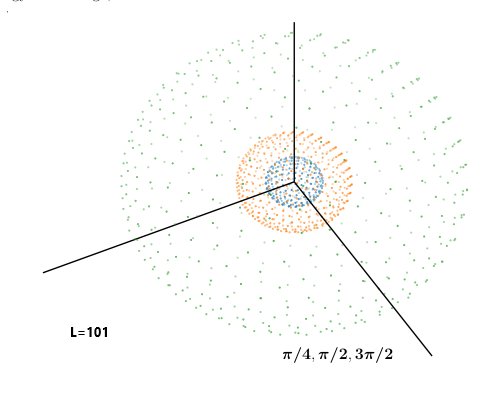
\includegraphics{fig1}}
\end{center}
\caption{The emergent $r\cdot\sin(r)$ wave cloud.}
\footnotesize{The cell-by-cell wave amplitude follows $\sin(r)/r$, while the number of cells per spherical shell scales as $r^{2}$; their product gives the radial interaction density $r\cdot\sin(r)$ used for electromagnetic coupling.}
\label{fig:wave-cloud}
\end{figure}

\subsection{Emergent polarization pair $(\mathrm{pol}_u,\mathrm{pol}_v)$}\label{subsec:polarization-pair}
Each active cell carries an integer pair $(u,v)$, stored as $\mathrm{pol}_u$ and $\mathrm{pol}_v$, that represents the transverse polarization in the plane tangent to the spherical wavefront.  The pair is not a geometric function of the local radius; it is derived from the \emph{broadcasted arrival stamp $b(x)$ of an elected momentum vector}.  At every turn-around of the breathing wavefront the automaton elects one direction out of its own state, a helical walker broadcasts the news of that election across the layer, and every cell converts its private arrival stamp into a polarization phase.  The mechanism has three stages---election, broadcast, and reconstruction---and uses only addition, subtraction, shift, and comparison.

\emph{Election.}  Every cell owns a predefined value $\nu\in[\,0,\,9L-1\,]$---its $W$-island index, fixed once by the internal address---and at the expansion limit of the pulse (the exact tick where the wave turns from ascending to descending) every active shell cell is seeded with the payload
\[
\mathrm{payload}(x)=\bigl(\mathrm{score}(x)\ll 24\bigr)\,\big|\,\mathrm{code}(x),
\qquad
\mathrm{score}=H\bigl((\nu(x)+s)\bmod 9L,\;\mathrm{code}(x)\bigr),
\]
where $\mathrm{code}(x)$ is the cell's linear index, $H$ a fixed integer hash, and $s$ a global seed dial.  Because the code occupies the low bits, the payload order is a strict total order: ties are impossible, so the winner is unique and independent of any scan order.  Each pass lets every cell adopt the greatest payload among its six face neighbours,
\[
\mathrm{payload}(x)\;\leftarrow\;\max\bigl(\mathrm{payload}(x),\;\mathrm{payload}(x\pm e_i)\bigr),
\]
with alternating sweep directions; $2R+8$ passes guarantee full coverage of the lattice.  The true winner---the \emph{seeded} cell holding the greatest payload---is identified once, at sowing time, while the payloads are still unique; the diffusion flood merely transports the news and never redefines the winner.  The displacement from the lattice center to the winning cell becomes the momentum vector $\boldsymbol{m}$, of which only the direction is meaningful: it is rescaled to $|\boldsymbol{m}|=L/2$ and frozen while the helical walk lives.  The next expansion limit elects a fresh direction for the next run; nothing is prescribed, and the orientation is read off the automaton's own ledger at the instant the wave reaches its limit.

\emph{Broadcast.}  As soon as $\boldsymbol{m}$ exists, a helical walker traces the spiral arm on the pulsating bubble.  It advances one cell per tick around the cylinder whose axis is the elected direction, keeping the radial error within about one cell by purely local comparisons among its six neighbours.  The walker is the arbitrary-axis integer helix ported from \texttt{spiral/spiral.c}: at election time it computes the constant cross products $\boldsymbol{D}_{m}=\boldsymbol{e}_{m}\times\boldsymbol{m}$, the shift tables $K_{km}=2\,\boldsymbol{D}_{k}\cdot\boldsymbol{D}_{m}$, the target radius $T_{\mathrm{GT}}=R_{\mathrm{CYL}}^{2}\,|\boldsymbol{m}|^{2}$ and the tolerance band $T_{\mathrm{OL}}=(2R_{\mathrm{CYL}}+1)\,|\boldsymbol{m}|^{2}$.  The cylinder radius is $R_{\mathrm{CYL}}=(93\,R_{\max}+256)/512$.  During the walk the squared radial error $E$, the direction filters $G_{m}$, and the orbital displacement $\boldsymbol{v}$ (with $q^{2}=|\boldsymbol{v}|^{2}$) are updated incrementally by addition, subtraction and shifts; an orbital step is chosen in the six-neighbour direction that keeps turning around $\boldsymbol{m}$ while staying inside the tolerance band, and a climb step along $\boldsymbol{m}$ is distributed by Bresenham so the walker also advances along the axis.

Each newly computed spiral point writes one plus the current tick into its own cell of a second value lattice, reserving $b(x)=0$ for ``never reached''.  Every other tick, with alternating sweep directions, every cell inspects only its six face neighbours and copies the greatest neighbour value whenever it exceeds its own,
\[
b(x)\;\leftarrow\;\max\bigl(b(x),\;b(x\pm e_i)\bigr).
\]
No cell ever senses beyond its neighborhood, yet these monotonic values diffuse as waves that in finite time reach every cell of the lattice---global coverage achieved purely by local moves, in lockstep with the automaton tick.  Each cell therefore ends up holding the tick $b(x)$ at which the news of the elected momentum arrived.

\emph{Reconstruction.}  The arrival stamp is the phase source.  A full $2\pi$ turn is encoded by $\mathrm{phase\_full}=2R^{2}$ units, where $R=L/2-2$ is the emergent bubble radius ($R$ and $\mathrm{phase\_full}$ are topological constants, Sect.~\ref{subsec:purity}), and the cell phase is read directly from the broadcasted value,
\[
\mathrm{cell\_phase}=(b(x)-1)\bmod\mathrm{phase\_full}, \qquad j=\left\lfloor\frac{\mathrm{cell\_phase}}{R}\right\rfloor .
\]
Writing $j_{2}=j-R$ for $j\ge R$, the integer pair is reconstructed by
\begin{align}
\text{if }j<R:\quad&u=R(R-2j),          &&v=2R\,\mathrm{isqrt}\bigl(j(R-j)\bigr),\\
\text{if }j\ge R:\quad&u=R(2j-3R),       &&v=-2R\,\mathrm{isqrt}\bigl(j_{2}(R-j_{2})\bigr).
\end{align}
These formulas generate an integer pair $(u,v)$ that lies on the integer lattice closest to the circle $u^{2}+v^{2}=R^{4}$ of radius $R^{2}$ (the equality is exact when the integer square root is exact, and is otherwise the closest integer approximation).  The polarization angle, defined geometrically as $\theta=\operatorname{atan2}(v,u)$, advances from $0$ to $2\pi$ as the broadcasted value grows, winding the polarization helix around the elected momentum axis.  This angle is never numerically evaluated by the automaton: it is the continuous geometric interpretation of the integer pair $(u,v)$, which encodes the direction implicitly.  No trigonometric tables, no precomputed spiral, and no per-cell fixed constants are used: the direction emerges from the tournament over the $W$-ledger, and the phase from the integer square-root relation applied to the arrival time.  Per the purity constraints (Sect.~\ref{subsec:purity}), the runtime performs no trigonometric computation whatsoever; $\operatorname{atan2}$ is introduced here only as a descriptor linking the integer pair to its emergent angular variable.

Once these fields are present, the cyclic evolution described in Sect.~\ref{sec:light-frame} begins.  Within that structured loop particles move, interact, and display emergent physical behavior.

%%%%%%%% THE LIGHT FRAME %%%%%%%%%%

\section{The light frame}\label{sec:light-frame}

The light frame (Figure \ref{fig:light_frame}) is one complete light step of the cellular automaton. It is divided into five stages: \texttt{CONVOL} (interactions and pair formation), \texttt{DIFFUSION} (propagation of contact, collapse, and translation information), \texttt{RELOC} (physical displacement of source centers), \texttt{REISSUE} (re-emission of the wavefront from the new source center), and \texttt{FLOOD} (final synchronization of the three lattices). The global housekeeping counter $k$ advances synchronously in every cell, marking the current stage; the wavefront counter $t$ is local and resets to zero whenever a bubble is reissued. The separation between the common $k$ and the local $t$ is what lets the finite-state machine coordinate essentially non-local operations while keeping them strictly non-signaling: no information and no influence ever travels faster than the maximum information speed $v_{\max}$, and causality is protected.

Despite its name, the light frame is not a unit of light propagation: it is the period of the information clock, within which a wavefront advances exactly one lattice cell, i.e. at the maximum speed of information transmission $v_{\max}$ (Sect.~\ref{sec:Results}). The speed of light does not appear anywhere in the transition rule; it is emergent. An Observer (Sect.~\ref{subsec:observers}) that measures distances and times by the round-trip convention of Sect.~\ref{subsec:special-relativity} reads the photon of Sect.~\ref{subsec:pairs}---a pair of bubbles riding the wavefront---as propagating at this speed and names it $c$. In particular, the \texttt{CONVOL} stage is superluminal in coordinate terms (it compares the whole lattice along $W$ in a single sweep), but it is strictly non-signaling and cannot be manipulated by any observer; causality is thereby protected.

\begin{figure}
\begin{center}

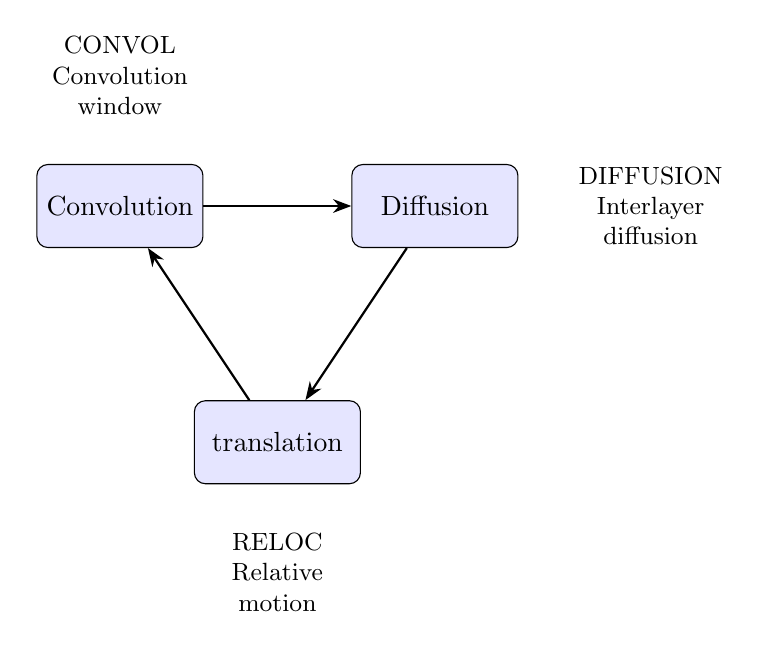
\begin{tikzpicture}[
    process/.style={rectangle, rounded corners, minimum height=3em, minimum width=6em, text centered, draw=black, fill=blue!10},
    arrow/.style={-Stealth, thick},
    annotation/.style={text width=6em, font=\small, align=center}
]

% Define the nodes for each step (3 boxes only)
\node[process] (convolution) at (0,0) {Convolution};
\node[process] (diffusion) at (4,0) {Diffusion};
\node[process] (translation) at (2,-3) {translation};

% Draw arrows to indicate the cyclic process (triangle shape)
\draw[arrow] (convolution) -- (diffusion);
\draw[arrow] (diffusion) -- (translation);
\draw[arrow] (translation) -- (convolution);

% Add annotations for constants
\node[annotation, above=0.5cm of convolution] (convol-anno) {CONVOL\\ Convolution window};
\node[annotation, right=0.5cm of diffusion] (diff-anno) {DIFFUSION\\ Interlayer diffusion};
\node[annotation, below=0.5cm of translation] (reloc-anno) {RELOC\\ Relative motion};

\end{tikzpicture}
\end{center}

\caption{The light frame---the period of the information clock, within which a wavefront advances exactly one lattice cell at the maximum information speed $v_{\max}$---has three stages: Convolution, Diffusion and translation, delimited by the constants CONVOL, DIFFUSION and RELOC.}
\label{fig:light_frame}
\end{figure}

\subsection{Definitions\label{subsec:Definitions}}

The frame constants are:

\begin{itemize}
\item \textbf{DIAG}\\
$\lfloor\sqrt{3}\,L\rfloor$: diagonal length of the lattice; upper bound for interaction distances.

\item \textbf{RMAX}\\
$L/2$: maximum bubble radius before wrapping (the breathing-phase amplitude).

\item \textbf{CONVOL}\\
$2W$: convolution window.

\item \textbf{DIFFUSION} \\
$CONVOL + 2W + \lfloor\sqrt{3}(L-1)/2\rfloor + 9(L-1) + 2W$: diffusion range along $W$; also alerts all layers of an imminent collapse.

\item \textbf{RELOC}\\
$DIFFUSION + 3(L-1)$: translation phase.

\item \textbf{REISSUE}\\
$RELOC + 1$: re-emission of the wavefront from the new source center.

\item \textbf{FLOOD}\\
$REISSUE + 3(L-1)$: final synchronization of the three lattices.

\item \textbf{FRAME}\\
Same value as $FLOOD$; total duration of the light step.

\item \textbf{effective\_t}\\
Triangular breathing phase (the active-shell radius): $\mathrm{effective\_t}(t)=t\bmod L$ for $t\bmod L\le L/2$, and $L-(t\bmod L)$ otherwise; period $L$, amplitude $L/2$.

\end{itemize}

\subsection{Bubble, pair, singleton, and blob} \label{subsec:pairs}

A \emph{bubble} is an expanding spherical wavefront of information organized across cells within a common layer. Spherical propagation is determined by comparing the dynamic radius $r$ to the wavefront tick $t$. 

\subsubsection{Pair}
Two bubbles are overlapping if they share the same spatial coordinates and $t_1=t_2$. Overlapping bubbles can form a \emph{pair} if they have the same affinity, that is, $a_1=a_2$; the two partners share a center and phase, and their charges are complementary or matching depending on the pair's role. Pairs may remain bound to a particle as \emph{dressing} pairs or propagate freely as photons; a free pair expands outward and is gradually consumed, releasing two singletons at distinct locations.

\subsubsection{Propeller} \label{subsubsec:propeller}
A pair can act as a \textit{propeller}, repositioning other bubbles and providing inertia.

\subsubsection{Singleton}
An unpaired bubble is called a \textit{singleton}; it is not a generic synonym for bubble.

\subsubsection{Blob}
The \textit{blob} is a group of superposed pairs having the same affinity, same true $bB$ bits and the same (active) pBits.

\subsubsection{Specialized pairs} \label{subsec:specialized-pairs}
Certain pair combinations are not allowed to form blobs: 

\begin{itemize}
    \item Neutrino and antineutrino pairs possess color values $N, N$ and $\bar{N}, \bar{N}$, respectively.

    \item The up quark fragments $u$ exhibit equal, nontrivial colors and a positive charge in the case of Orbis. 

    \item The propeller adds to the relativistic mass of the propelled fermion.\footnote{This mirrors a Kantian view: particles do not self-move but require an external cause—here, interaction with fragments—to change their state.}

    \item Pairs with fully complementary charges are \emph{gravitons}. They operate in both Orbis and Umbra,\footnote{Orbis and Umbra coexist spatially.} have fixed oscillation frequency $2$, and mediate static cross-sector interactions; without them, Umbra matter would appear inert in Orbis. Graviton-induced gravity is detailed in Sect.~\ref{subsec:emergence-of-gravity}.
\end{itemize}

\subsection{Interaction principles}
The guiding principles are:

\subsubsection{Wavefronts clash}
The wavefronts of both bubbles must be active, i.e. $r_1 = \mathrm{effective\_t}(t_1)$ and $r_2 = \mathrm{effective\_t}(t_2)$, where $r_i$ is the propagated integer radius of bubble $i$ and $t_i$ is its local frame counter. This condition is assumed in all rules below.

\subsubsection{Aggregation and dissolution}\label{subsec-role-of-affinity}

Bubbles aggregate by sharing a common affinity; the smallest value prevails, $a_1=a_2=\min(a_1,a_2)$. On dissolution, they revert to their layer indices, $a_1=w_1$ and $a_2=w_2$. If a singleton meets a pair, the pair takes the singleton's affinity, $a_2^1=a_2^2=a_1$. The value $a=W$ marks an orphan. The idempotent $\min$ operator naturally supports an ontological model of entanglement.

\subsubsection{Charge conjugation}

Charge conjugation constrains interactions by requiring charge neutrality in the outcome. Electric neutrality requires a pair of opposite charges; a single bit cannot be neutral alone. Weak neutrality follows from the combination of the two weak bits in both \textit{Orbis} and \textit{Umbra}. Strong neutrality is $000$ (or $111$ for anti-neutrality); a pair with complementary color bits (e.g. $101$ and $010$) is also neutral. In general, interactions drive the resulting charge combination toward neutrality.

\subsubsection{Reciprocity}
Because only one draft can be updated at a time, the rules must later update the counterpart. This reciprocity is essential for the next subsection.

\subsection{Convolution} \label{subsec:convolution}
Convolution is the first step of the light frame (ending at $CONVOL$) and contains the main interaction rules. Each site in the main lattice is compared with its mirror along the $W$ dimension. This mirror comparison is a rule-evaluation device that pairs lattice sites by internal address; it does not move bubbles along $W$---physical motion and merging always occur in the 3-torus (Sect.~\ref{subsec:w-islands}). During this step the wave phase $f$ (the triangular breathing phase of Sect.~\ref{sec:light-frame}) selects the wave-cloud point density at the current shell, while the notion of frequency is carried by the pair count (Sect.~\ref{bosons}). Particles form or reform here. We postulate that the weak force only causes collapse, not limited reissues. Comparisons split into two cases: superposing or distinct bubbles.

\subsubsection{Superposing bubbles}
Two overlapping bubbles with the same wavefront tick $t_1=t_2$ can form a pair if they satisfy the following conditions:
\begin{itemize}
% Rule 1
\item
$ (q_a \oplus q_b) \land (w1_a \oplus w1_b) \land (w0_a \oplus w0_b) \land (c2_a \oplus c2_b) \land (c1_a \oplus c1_b) \land (c0_a \oplus c0_b) $
\item

% Rule 2
$ (q_a \oplus q_b) \land (w1_a = w1_b) \land (w0_a \oplus w0_b) \land (c2_a \oplus c2_b) \land (c1_a \oplus c1_b) \land (c0_a \oplus c0_b) $
\item

% TODO: add the gluon and weak boson formation rules
% Rule 3
$ ch_a = ch_b = 000000\mathrm{B} $
\item

% Rule 4
$ ch_a = ch_b = 111111\mathrm{B} $
\item

% Rule 5
$ (q_a = q_b = 0) \land (w1_a = w1_b = 0) \land (w0_a = w0_b = 1) \land (color_a = color_b) \land (color_a \neq 000\mathrm{B} \land color_a \neq 111\mathrm{B}) $
\item

% Rule 6
$ (q_a = q_b = 1) \land (w1_a = w1_b = 1) \land (w0_a = w0_b = 0) \land (color_a = color_b) \land (color_a \neq 000\mathrm{B} \land color_a \neq 111\mathrm{B}) $

\end{itemize}

To make the six rules concrete, Table~\ref{tab:charge-examples} lists representative bit-strings (written in the order $w_{1}\,w_{0}\,q\,c_{2}\,c_{1}\,c_{0}$ of Table~\ref{tab:Cell-structure}) and the pairs they form.  Colors follow the code of Table~\ref{tab:Cell-structure}: $N=000$, $R=001$, $G=010$, $\bar{B}=011$, $B=100$, $\bar{G}=101$, $\bar{R}=110$, $\bar{N}=111$.

\begin{table}[h]
\centering
\caption{Representative charge bit-strings and the pairs they form under rules R1--R6.}
\label{tab:charge-examples}
\begin{tabular}{|c|c|c|l|}
\hline
Rule & bubble $a$ & bubble $b$ & pair formed\\
\hline
R1 & $011001$ & $100110$ & graviton (all six bits complementary)\\
R2 & $011001$ & $000110$ & gluon ($w_1$ equal, $q/w_0$/colour complementary)\\
R3 & $000000$ & $000000$ & neutrino\\
R4 & $111111$ & $111111$ & antineutrino\\
R5 & $010001$ & $010001$ & up quark ($q{=}0$, $w_1{=}0$, $w_0{=}1$, colour $R$)\\
R6 & $110001$ & $110001$ & up quark ($q{=}1$, $w_1{=}1$, $w_0{=}0$, colour $R$)\\
\hline
\end{tabular}
\end{table}

These rules implement the formation of pairs, as defined in Sect. \ref{subsec:pairs}. 
If pairs are detected, one frequency unit is registered on the pair stack (Sect.~\ref{bosons}); the wave phase $f$ itself remains the triangular breathing phase of the local tick.
$s2B$ is updated as $s2B' = s2B \ \textbf{and} \ \mathit{active}$. 
Notice that the pairs are formed in two steps: first, cell $a$ compares with cell $b$, and later, cell $b$ compares with cell $a$ (reciprocity).
The formation of blobs is made during this step too, also following the reciprocity principle. 

Pairs are allowed to superpose if they are equal and were formed by the two first rules above.

\subsubsection{Distinct bubbles} \label{subsec:distinct}
The $w_1$ bit separates distinct-bubble interactions into same-sector ($w_1^1=w_1^2$) and inter-sector cases; we first treat same-sector interactions.

If two same-sector singletons have opposite charges and both $kB$ bits false, we have annihilation, with both bubbles being reissued from the contact point and their affinity receiving their default values. The draft $kB$ bit turns true, triggering a collapse.

Else if two singletons have the same charge, we have fermion cohesion. 
One bubble is reissued from the contact point, while the other, from its active $sB$ site. 
Also, they become entangled ($a_1=a_2$).

On the other hand, if the two bubbles share the same affinity, but have different charges, the bubble whose wavefront at the contact point has $pB=1$ is reissued from the contact point.
The other bubble is reissued using the inertial-transported translation impulse, accumulated in the vector $\boldsymbol{\mathit{reloc}}$; the stable momentum vector $\boldsymbol{m}$ supplies the direction of that impulse, while the translation vector $\boldsymbol{c}$ is consumed during the reissue step.
That is, one bubble is reissued from $\boldsymbol{x1}$, while the other from $(\boldsymbol{x_1}-\boldsymbol{x_2})\,\boldsymbol{mod}\,L$.

For color-neutral combinations there are two cases: gluon$\times$gluon and quark$\times$gluon. 
In both cases, the two bubbles are reissued from the contact point and the partners colors are exchanged.

In the electroweak sector, both $\mathit{active}$ bits must be true; together with $s2B$ they determine the harmonic behavior. This sieve mechanism applies only to electroweak interactions and helps explain why the strong force is stronger.

The weak interaction occurs when the weak charges are combined to neutrality and either ($pB_1=1$, $pB_2=0$) or ($sB_1=sB_2=1$); it always triggers collapse ($kB=1$).

The electric case uses one $pB$ bit, the magnetic case one $sB$ bit. If both $pB$ bits are true (or both $sB$ bits in the magnetic case), a collapse is triggered ($kB=1$).

If only one $pB$ bit meets the other's surface, the interaction is adiabatic: no collapse occurs, but the bubbles exchange affinity and time and relocate to each other's center. The $a$ and $t$ values then spread throughout the layer.

At the initial singularity, all bubbles overlap. If two bubbles belong to different sectors and $t=RMAX/2$, they are reissued from their active $pB$ and $sB$ sites, dispersing the singularity and separating Orbis from Umbra. We call this \textit{dispersion}.

\subsubsection{Inter-sector interactions}
For inter-sector interactions, fully complementary charges lead to \textit{singularization}; otherwise the electroweak rules above apply. Singularization is the counterpart to dispersion. 
The bubbles are reissued from the contact point ($pB_{curr}=\text{true}$).

%%% DIFFUSION %%%

\subsection{Diffusion}

Diffusion propagates the information needed for translation, ending at the \texttt{DIFFUSION} tick (Figure~\ref{fig:diffusion}). If any collapse bit $kB$ is set, it spreads to all bubbles sharing the same affinity, identifying every contributor to the collapsing particle.

The wave phase $f$ is not diffused: it is the local triangular breathing phase $\mathrm{effective\_t}(t)$ of each cell (Sect.~\ref{sec:light-frame}). Phases incremented by multiples of the fundamental cycle interact with the wave-cloud sieve to form concentric bubbles; the active wavefront point ($t=d$) is forwarded to the Euclidean bubble through $s2B$.

At the same time, the translation vector $\mathbf{c}$ diffuses through the layer: each cell copies the first non-trivial $\mathbf{c}$ found among its neighbors. Finally, $sB$ hunting increments $\boldsymbol{c}$ along any axis where a neighbor has $hB=1$, but only when the local cell has $sB=0$. By the end of diffusion, $\boldsymbol{c}$ is ready for translation.


\begin{figure}
\begin{center}

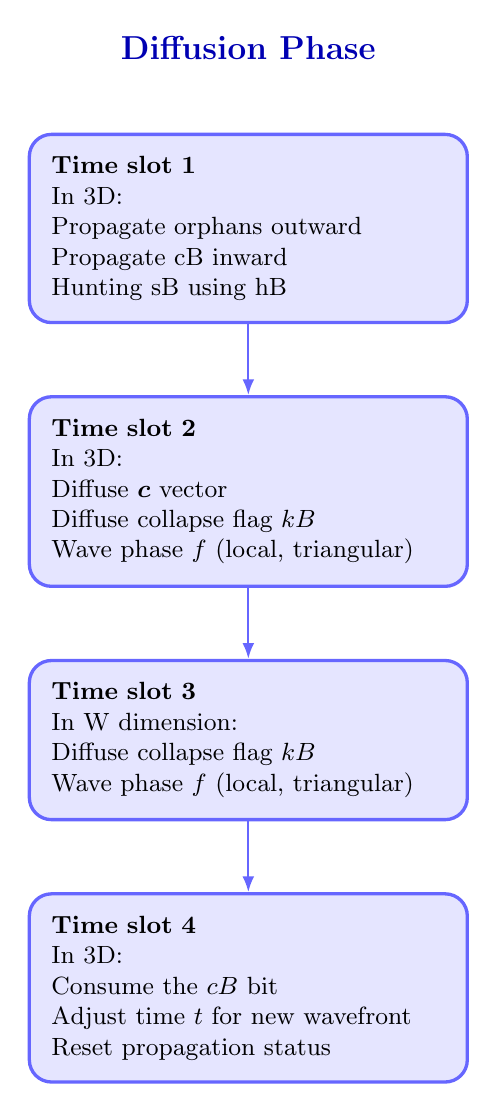
\begin{tikzpicture}[
  every node/.style={font=\small, align=left},
  phase/.style={rectangle, rounded corners=8pt, draw=blue!60, fill=blue!10, very thick, text width=5cm, inner sep=8pt},
  arrow/.style={-{Latex[length=2mm]}, thick, blue!60}
]

% Nodes (closer spacing)
\node[phase] (t1) {
  \textbf{Time slot 1}\\
  In 3D:\\
  Propagate orphans outward\\
  Propagate cB inward\\
  Hunting sB using hB
};

\node[phase, below=0.9cm of t1] (t2) {
  \textbf{Time slot 2}\\
  In 3D:\\
  Diffuse $\boldsymbol{c}$ vector\\
  Diffuse collapse flag $kB$\\
  Wave phase $f$ (local, triangular)
};

\node[phase, below=0.9cm of t2] (t3) {
  \textbf{Time slot 3}\\
  In W dimension:\\
  Diffuse collapse flag $kB$\\
  Wave phase $f$ (local, triangular)
};

\node[phase, below=0.9cm of t3] (t4) {
  \textbf{Time slot 4}\\
  In 3D:\\
  Consume the $cB$ bit\\
  Adjust time $t$ for new wavefront\\
  Reset propagation status
};

% Shorter arrows
\draw[arrow] (t1.south) -- ++(0,-0.25) -> (t2.north);
\draw[arrow] (t2.south) -- ++(0,-0.25) -> (t3.north);
\draw[arrow] (t3.south) -- ++(0,-0.25) -> (t4.north);

% Title
\node[above=0.8cm of t1, font=\bfseries\large, blue!70!black] {Diffusion Phase};

\end{tikzpicture}
\end{center}
\caption{The Diffusion phase is composed of several time slots. It spreads all information necessary for translation.}
\label{fig:diffusion}
\end{figure}

%%% translation %%%
\subsection{translation} \label{subsec:translation}
This part of the light step addresses bubble translation itself, building on the diffusion step. 
It ends at the RELOC tick. Bubbles shift in specific directions (north, west, down) until they have completed their translation process, including the inertial transport mechanism. 
The example rule is: if $\textbf{c}_x^{north}>0$, copy the content of the neighbor cell to the draft cell and decrement $\textbf{c}_x$ at the draft cell.

Since wavefront propagation is guided by the dynamic radius $r$ propagated from the source cell, when a bubble is re-emitted due to interaction with other bubbles, all pertinent cell information must be shifted, or relocated, to the new position determined by the variable $\textbf{c}$. 
This ensures that the bubbles are relatively displaced from each other. 
The final operation sets $t=0$ at the center cell of the relocated pattern. 
translation is the main consequence of an interaction.

Bubbles are re-emitted either immediately after an interaction or through wrapping. 
When the bubble is reissued, the previous wavefront continues to propagate until it fades through wrapping. 
In this state, the bubble is referred to as an \textit{orphan}, meaning it has affinity disabled but is still capable of non-collapsing interactions. 
In this case, $a=W$ for the outer cells, set during the translation step. 

To complete, the diffusion of the time variable $t$ occurs here at the last tick: When a cell has a neighboring cell with a lower $t$ value, it updates its own $t$ variable to match the lower value. 
With this rule, the relocated bubble is capable of expanding again. 
This timing is crucial to avoid the 'clean diamond' pattern with the new values overrunning the orphaned data.

When the translation is complete, bubble variables are prepared for the next cycle. 
If the time frame completes, the $k$ counter resets to zero, preparing the system for the next iteration.  
At the conclusion of the process, all $\boldsymbol{c}$ vectors will have a null value.

A propeller ($P$) can only be relocated to a point on its active surface. In a $P \times K$, $P \times D$ or $P \times S$ interaction, the $P$ source is reissued from the active contact cell where the two wavefronts overlap; this contact point is already reached at the maximum information speed $v_{\max}$, so no superluminal transfer of information is required---the convolution that reads the contact is itself superluminal in coordinate speed but strictly non-signaling.

Inertia is acquired by an inertial-transport mechanism. The propeller transfers its stable momentum direction $\boldsymbol{m}$ to the partner's consumable translation impulse $\boldsymbol{\mathit{reloc}}$; during the next light step the partner's source center is shifted by $\boldsymbol{\mathit{reloc}}$, while its long-term $\boldsymbol{m}$ is preserved and updated by \texttt{applyMomentum()}.
The $P$ source itself is reissued from the contact point; the partner ($K$, $D$ or $S$) keeps its source kind but receives the impulse.
A single propeller kick acts on one bubble at a time: only the contacted partner source receives $\boldsymbol{\mathit{reloc}}$, while all other bubbles of the aggregate keep their centers. Let $N$ be the total number of bubbles composing the particle (the $3$D island plus its pair dressing). If $n$ bubbles receive an impulse during one light frame, the mean center of mass advances by
\begin{equation}
\Delta_{\mathrm{CoM}} \;=\; \frac{n}{N}
\end{equation}
cells per frame, with $n \leq N$. Sub-luminal motion is therefore structural: a larger population responds less to the same kick rate — the discrete counterpart of propeller contributions to mass — whereas a photon blob, whose superposed pairs share a single center, attains $n/N \to 1$. When no kick arrives ($\boldsymbol{\mathit{reloc}}=\boldsymbol{0}$) the particle merely breathes at rest.

Non-propeller pairs behave differently: in $K \times K$ or $D \times D$ between different tribes the source centers move one light-step away from each other, exchanging momentum through $\boldsymbol{\mathit{reloc}}$.

The propeller (Sect.~\ref{subsubsec:propeller}) is a pair ($P$) that acts as a carrier of momentum. Free photon or graviton pairs may become propellers through the same $P$ source mechanism, but during interaction the source kind $P$ is treated as a single relocating source whose momentum is transferred to the non-$P$ partner.

\subsection{Annihilation and collapse}

Annihilation and light-matter collapse both occur during convolution. In annihilation, the affinity reverts to its default value $a=w$, and the resulting bubbles become raw material for new particles.

This ontological collapse introduces an arrow of time at the fundamental level, reinforcing the second law of thermodynamics and pushing Poincaré recurrence far into the future (Sect.~\ref{sec-undecidability}).

\subsection{Main lattice updating and mirroring} \label{subsec:updating}
At the end of each $k$ tick, the draft lattice is transferred to main. If $k$ lies inside the $CONVOL$ window, draft is first shifted along $W$ to enable convolution. This shift is a cyclic permutation of internal addresses for evaluation, not propagation of bubbles along an extra spatial axis---all physical motion remains confined to the 3-torus (Sect.~\ref{subsec:w-islands}). The mirror lattice is then refreshed from main so the next convolution can compare main and mirror along $W$; it copies the wave phase and active flag, $f_i^{mirror}=f_i^{main}$ and $\mathit{active}_i^{mirror}=\mathit{active}_i^{main}$.

\subsection{Algorithmic summary of one light frame}\label{subsec:algorithm}

For reproducibility, Algorithms~\ref{alg:lightframe}--\ref{alg:blob} give a self-contained account of one complete light frame: Algorithm~\ref{alg:lightframe} is the frame driver (incremental distance field, integer wave update, the six interaction stages, the charge-conjugation hook, momentum and lattice swap), and Algorithms~\ref{alg:pair}--\ref{alg:blob} give the interaction rules invoked by the \textsc{Convolute} stage.  Together they define the full transition function; the repository (Ref.~\cite{af_neto}, \texttt{simulation.cpp}, \texttt{interaction.cpp}) is not needed to reproduce the dynamics.  The notation follows Table~\ref{tab:Cell-structure}: a charge word is written $w_{1}\,w_{0}\,q\,c_{2}\,c_{1}\,c_{0}$ (most significant first), $c_{2}c_{1}c_{0}$ is the colour, $000\mathrm{B}=N$ and $111\mathrm{B}=\bar{N}$, and $\overline{ca}$ denotes the six-bit complement of the charge word $ca$.  Subscripts $a$ and $b$ label the two interacting bubbles, so $q_a$ is bit $q$ of bubble $a$, $w_{1,a}$ bit $w_{1}$ of bubble $a$, and so on.

\begin{algorithm}[ht]
\caption{One complete light frame (the full per-cell transition function, one synchronous $k$-tick).}
\label{alg:lightframe}
\begin{algorithmic}[1]
\Require $L$, $W=3L^{2}$, $\mathrm{RMAX}=L/2$, and the stage bounds
  $\mathrm{CONVOL}<\mathrm{GSLOT\_Z}<\mathrm{DIFFUSION}<\mathrm{RELOC}<\mathrm{REISSUE}<\mathrm{FLOOD}=\mathrm{FRAME}$ (Sect.~\ref{subsec:Definitions});
  the housekeeping tick $k$, the wavefront tick $t$, and the wave phase $f=\mathrm{effective\_t}(t)$ are the cell fields of Table~\ref{tab:Cell-structure}
\Ensure the three lattices advanced by one light step
\Procedure{LightFrame}{}
  \State \Call{UpdatePulsatingWavefront}{} \Comment{incremental distance field: radii $r^{2},r$ from the moving source centre by $\Delta{=}2a{+}1$ increments, no square roots}
  \State $pulse\_tick \gets pulse\_tick + 1$
  \State \Call{PhaseStep}{} \Comment{integer wave update $v \gets v + (\nabla^{2}u \gg s)$, $u \gets u + v$, damping $v \gets v - (v \gg s_{d})$, shifts $s,s_{d}$ radius-dependent; hard zero outside the sphere; $active \Leftrightarrow r=\mathrm{effective\_t}(t)$}
  \State swap $lattice\_curr \leftrightarrow lattice\_draft$
  \State \Call{PolarizationTick}{} \Comment{elected-momentum broadcast over the $W$-ledger; stamps arrival ticks $b(x)$}
  \For{$w = 0 \ldots W{-}1$} \Comment{loop over the internal dimension}
    \For{each cell $(x,y,z)$ in the 3-torus}
      \State $C \gets lattice\_curr(x,y,z,w)$; $D \gets C$; $M \gets lattice\_mirror(x,y,z,w)$
      \If{$k < \mathrm{CONVOL}$}
        \State \Call{Convolute}{$C,D,M$} \Comment{interaction rules R1--R6, Algorithms~\ref{alg:pair}--\ref{alg:blob}; source-kind (K/S/D/P) contact re-emission and momentum impulse}
      \ElsIf{$k < \mathrm{GSLOT\_Z}$}
        \State glider slots \Comment{reserved for the antipodal transport schedule; no-op in the CPU reference path}
      \ElsIf{$k < \mathrm{DIFFUSION}$}
        \State \Call{Diffuse}{$C,D$} \Comment{orphan expansion ($a \gets W$ from a full neighbour); hunting $hB \to$ translation vector $\boldsymbol{c}$; $\boldsymbol{c}$ and $kB$ transport; affinity settle}
      \ElsIf{$k < \mathrm{RELOC}$}
        \State \Call{Relocate}{$C,D$} \Comment{consume the translation vector $\boldsymbol{c}$ along the three axes (north, west, down)}
      \ElsIf{$k < \mathrm{REISSUE}$}
        \State \Call{Reissue}{$C,D$} \Comment{reset $kB,hB,bB$; propagate affinity outward from $active$ cells; consume the contraction flag $cB$ (reset $t$)}
      \Else
        \State \Call{Flood}{$C,D$} \Comment{synchronize the light clock: $D.t \gets \min$ of the six neighbour $t$}
      \EndIf
      \State $D.k \gets (C.k + 1) \bmod \mathrm{FRAME}$
      \If{$D.k = 0$} \Comment{a new light frame begins}
        \State $D.t \gets (C.t + 1) \bmod (2\,\mathrm{RMAX})$ \Comment{island cells ($a{=}W$, $t \le \mathrm{RMAX}$) count without the modulus}
      \EndIf
    \EndFor
  \EndFor
  \State \Call{ApplyChargeConjugation}{} \Comment{matter--antimatter turnaround hook; exact no-op when the bias $\varepsilon = 0$}
  \State \Call{ApplyMomentum}{} \Comment{consume one photon pair at $t=\mathrm{RMAX}$, release singletons; advance source centres by $\boldsymbol{\mathit{reloc}}$; re-seed the pulsating wave at the new centre}
  \State \Call{SwapLattices}{} \Comment{$\mathrm{draft}\to\mathrm{curr}$; at $k=0$ refresh the mirror ($M.f \gets \mathrm{effective\_t}(M.t)$); while $k<\mathrm{CONVOL}$ rotate the mirror $W$-slices (\textsc{ShiftMirror})}
\EndProcedure
\end{algorithmic}
\end{algorithm}


\begin{algorithm}[ht]
\caption{Exact interaction rules for the six charge bits (superposing bubbles).}
\label{alg:pair}
\begin{algorithmic}[1]
\Function{CanFormPair}{$a,b$}
  \State $ca \gets a.ch$; $cb \gets b.ch$
  \If{$ca = 000000\mathrm{B}$ \textbf{and} $cb = 000000\mathrm{B}$} \Comment{R3: neutrino}
    \State \Return \textbf{true}
  \ElsIf{$ca = 111111\mathrm{B}$ \textbf{and} $cb = 111111\mathrm{B}$} \Comment{R4: antineutrino}
    \State \Return \textbf{true}
  \ElsIf{$\overline{ca} = cb$} \Comment{R1: graviton, all six bits complementary}
    \State \Return \textbf{true}
  \EndIf
  \State $(q_a,w_{1,a},w_{0,a}) \gets$ decode bits of $ca$; $(q_b,w_{1,b},w_{0,b}) \gets$ decode bits of $cb$
  \State $col_a \gets ca \& 111\mathrm{B}$; $col_b \gets cb \& 111\mathrm{B}$
  \If{$q_a \neq q_b$ \textbf{and} $w_{1,a} = w_{1,b}$ \textbf{and} $w_{0,a} \neq w_{0,b}$ \textbf{and} $col_a \oplus col_b = 111\mathrm{B}$} \Comment{R2: gluon}
    \State \Return \textbf{true}
  \ElsIf{$q_a = q_b = 0$ \textbf{and} $w_{1,a} = w_{1,b} = 0$ \textbf{and} $w_{0,a} = w_{0,b} = 1$ \textbf{and} $col_a = col_b$ \textbf{and} $col_a \notin \{000,111\}\mathrm{B}$} \Comment{R5: up quark}
    \State \Return \textbf{true}
  \ElsIf{$q_a = q_b = 1$ \textbf{and} $w_{1,a} = w_{1,b} = 1$ \textbf{and} $w_{0,a} = w_{0,b} = 0$ \textbf{and} $col_a = col_b$ \textbf{and} $col_a \notin \{000,111\}\mathrm{B}$} \Comment{R6: up quark}
    \State \Return \textbf{true}
  \EndIf
  \State \Return \textbf{false}
\EndFunction
\end{algorithmic}
\end{algorithm}


\begin{algorithm}[ht]
\caption{Blob formation, electric/magnetic channels, and collapse (superposing and distinct bubbles).}
\label{alg:blob}
\begin{algorithmic}[1]
\Function{CanFormBlob}{$a,b$}
  \State $ca \gets a.ch$; $cb \gets b.ch$
  \If{$ca = cb = 000000\mathrm{B}$ \textbf{or} $ca = cb = 111111\mathrm{B}$} \Comment{R3/R4 never blob}
    \State \Return \textbf{false}
  \ElsIf{$\overline{ca} = cb$} \Comment{R1 graviton never blobs}
    \State \Return \textbf{false}
  \EndIf
  \State decode $(q,w_{1},w_{0})$ and $col$ of $ca,cb$ as in Algorithm~\ref{alg:pair}
  \If{$q_a = q_b$ \textbf{and} $w_{1,a} = w_{1,b}$ \textbf{and} $w_{0,a} = w_{0,b}$ \textbf{and} $col_a = col_b$ \textbf{and} $col_a \notin \{000,111\}\mathrm{B}$} \Comment{R5/R6 up quark never blobs}
    \State \Return \textbf{false}
  \ElsIf{$a.\mathit{reloc} \neq 0$ \textbf{or} $b.\mathit{reloc} \neq 0$} \Comment{propeller never blobs}
    \State \Return \textbf{false}
  \EndIf
  \State \Return $w_{1,a} = w_{1,b}$ \textbf{and} $q_a \neq q_b$ \textbf{and} $w_{0,a} \neq w_{0,b}$ \textbf{and} $col_a \oplus col_b = 111\mathrm{B}$ \Comment{only the R2 geometry}
\EndFunction
\Procedure{Convolute}{$C,D,M$}
  \State $samePos \gets C.x = M.x$; $sameT \gets C.t = M.t$
  \If{$samePos$ \textbf{and} $sameT$ \textbf{and} \Call{CanFormPair}{$C,M$}}
    \State $D.kind \gets M.kind \gets P$; $D.pair\_idx \gets M.w$; $M.pair\_idx \gets C.w$ \Comment{form a pair}
    \State $D.a \gets M.a \gets$ shared affinity; \Call{ReemitAtContact}{$D,M$}; reset $t$
    \If{$newCount > 1$ \textbf{and} \Call{CanFormBlob}{$C,M$} \textbf{and} $C.pB = M.pB$ \textbf{and} $C.sB = M.sB$ \textbf{and} $C.bB = M.bB$}
      \State $D.bB \gets M.bB \gets \textbf{true}$ \Comment{blob}
    \EndIf
  \ElsIf{$C.pB$ \textbf{or} $M.pB$ \textbf{or} $C.sB$ \textbf{or} $M.sB$} \Comment{electric/magnetic contact}
    \If{$C.pB \wedge M.pB$ \textbf{or} $C.sB \wedge M.sB$} \Comment{collapse}
      \State $D.kB \gets D.cB \gets \textbf{true}$ \Comment{triggers reissue}
    \Else
      \State \Call{AdiabaticExchange}{$C,D,M$} \Comment{exchange affinity and phase, relocate to partner center}
\EndIf
  \EndIf
\EndProcedure
\end{algorithmic}
\end{algorithm}

As given in Sect.~\ref{subsec:updating}, \textsc{SwapLattices} transfers the draft to the main lattice at the end of every $k$ tick; at $k=0$ the mirror is refreshed from main (so the next convolution compares main and mirror along $W$), and while $k<\mathrm{CONVOL}$ the mirror $W$-slices are rotated by \textsc{ShiftMirror} to schedule the cross-layer adjacency.

%%%%%%%% INTERACTIONS %%%%%%%%%%

\section{Interactions\label{sec:Interactions}}

Some interaction details are now clarified.

\subsection{Charge driven interactions}


\subsubsection{Static interactions}

A static interaction (Coulomb or magnetic) between two distant charges $q_1$ and $q_2$ begins when an orphan singleton from $q_1$ aligns with a vacuum graviton; both are reissued at the contact point. If the graviton then interacts with $q_2$, it is reissued there and acquires $q_2$'s affinity. Thus gravitons propagate along the flux of orphans from particle 1, increasing the chance of hitting $q_2$ and becoming one of its propellers. The same occurs in reverse.

\subsubsection{Coulomb interaction} \label{subsec:Coulomb-interaction}

Coulomb attraction and repulsion occur in two steps: (a) the wavefront of an orphan from the first charge, with $pB=1$, contacts an active cell of a graviton; if their position vectors are aligned or anti-aligned, the graviton is reissued from the contact point with the orphan's affinity; (b) the second charge's wavefront, also with $pB=1$, contacts the reissued graviton and receives a translation impulse in the direction of its momentum vector $\boldsymbol{m}$, becoming a propeller pointing in the correct direction.

\subsubsection{Static magnetic interaction}

The magnetic case uses $sB$ instead of $pB$ and applies to charged leptons, quarks and W bosons. Because propellers emphasize $pB$ over $sB$, fast particles tend to acquire a component perpendicular to their direction of motion.

\subsubsection{Neutrino interactions}

Let $q_{0,1}$ be a complementary electric-bit pair. A neutrino fragment has charge content $q_{0,1}=00000B$; an antineutrino has $q_{0,1}=01111B$. (Anti)neutrino fragments interact only with (right-)left-handed particles.

\subsubsection{The up quark and down quark fragments}

The color combinations of fragment pairs are shown in Table~\ref{tab:color-combination}. 
(Anti)\emph{quark} fragments have non-trivial color and are marked as $1q$ or $1\bar{q}$, (anti)neutrinos are $\nu$ and $\bar{\nu}$, gluons are $g$, and photons are $\gamma$. 
Since half the gluon fragments are right-handed, they are shown as photons. 
The shaded cells (same-colour pairs) with both quarks carrying electric charge $q=+$ may form an \emph{up quark} fragment. 

An \emph{up quark} $u$ can be any of the \emph{+R+R}, \emph{+G+G} or \emph{+B+B} pairs, while a \emph{down quark} $d$ can be any of the \emph{-R}, \emph{-G} or \emph{-B} single fragments. A proton fragment \emph{uud} has an uncompensated color, balanced dynamically by the matter and antimatter ends of gluons. Hence the \emph{electron} fragment must be $-N,-N,-N$.\footnote{This explains fractional quark charges.}

The number of up-quark fragments in each sector sets an upper limit on proton, and hence \textit{atom}, production.

\subsection{Self-interference\label{subsec:Interference}}

Space in this model retains a memory of particle trajectories, producing self-interference reminiscent of the double-slit experiment \cite{feynman-2}. The trace is encoded by the last affinity value $a$ and the most recent wave phase $f$ left in visited cells.

During convolution (Sect.~\ref{subsec:convolution}), incoming and residual bubbles are compared. If $d=t$, standard cohesion occurs; if $d=f$, only the new bubble is reissued, altering the fermion's dynamics and creating interference patterns. This temporally shifted interaction among the constituent ``bits'' of qubits (Sect.~\ref{subsection:qubits}) provides a substrate for complex quantum behavior in a discrete framework.


\begin{table}[p]
\centering
\setlength{\tabcolsep}{2.2pt}
\renewcommand{\arraystretch}{0.95}
\resizebox{0.72\linewidth}{!}{%
\begin{tabular}{|c|c|c|c|c|c|c|c|c|}
\hline
 &
 \hdr{N}{000} &
 \hdr{R}{001} &
 \hdr{G}{010} &
 \hdr{$\bar{\mathrm{B}}$}{011} &
 \hdr{B}{100} &
 \hdr{$\bar{\mathrm{G}}$}{101} &
 \hdr{$\bar{\mathrm{R}}$}{110} &
 \hdr{$\bar{\mathrm{N}}$}{111} \\
\hline
% N 000
\hdr{N}{000} &
  \C{\nu} &
  \Csec{1q}{1\ell} &
  \Csec{1q}{1\ell} &
  \Csec{1\overline{q}}{1\ell} &
  \Csec{1q}{1\ell} &
  \Csec{1\overline{q}}{1\ell} &
  \Csec{1\overline{q}}{1\ell} &
  \C{\gamma} \\
\hline
% R 001
\hdr{R}{001} &
  \Csec{1\ell}{1q} &
  \Cb{2q} &
  \C{2q} &
  \C{\gamma} &
  \C{2q} &
  \C{\gamma} &
  \C{\gamma} &
  \Csec{1\overline{\ell}}{1q} \\
\hline
% G 010
\hdr{G}{010} &
  \Csec{1\ell}{1q} &
  \C{2q} &
  \Cb{2q} &
  \C{g} &
  \C{2q} &
  \C{\gamma} &
  \C{\gamma} &
  \Csec{1\overline{\ell}}{1q} \\
\hline
% B-bar 011
\hdr{$\bar{\mathrm{B}}$}{011} &
  \Csec{1\ell}{1\overline{q}} &
  \C{g} &
  \C{g} &
  \Cy{2\overline{q}} &
  \C{g} &
  \C{2\overline{q}} &
  \C{2\overline{q}} &
  \Csec{1\overline{\ell}}{1\overline{q}} \\
\hline
% B 100
\hdr{B}{100} &
  \Csec{1\ell}{1q} &
  \C{2q} &
  \C{2q} &
  \C{g} &
  \Cb{2q} &
  \C{\gamma} &
  \C{\gamma} &
  \Csec{1\overline{\ell}}{1q} \\
\hline
% G-bar 101
\hdr{$\bar{\mathrm{G}}$}{101} &
  \Csec{1\ell}{1\overline{q}} &
  \C{g} &
  \C{g} &
  \C{2\overline{q}} &
  \C{\gamma} &
  \Cy{2\overline{q}} &
  \C{2\overline{q}} &
  \Csec{1\overline{\ell}}{1\overline{q}} \\
\hline
% R-bar 110
\hdr{$\bar{\mathrm{R}}$}{110} &
  \Csec{1\ell}{1\overline{q}} &
  \C{g} &
  \C{g} &
  \C{2\overline{q}} &
  \C{\gamma} &
  \C{2\overline{q}} &
  \Cy{2\overline{q}} &
  \Csec{1\overline{\ell}}{1\overline{q}} \\
\hline
% N-bar 111
\hdr{$\bar{\mathrm{N}}$}{111} &
  \C{\gamma} &
  \Csec{1q}{1\overline{\ell}} &
  \Csec{1q}{1\overline{\ell}} &
  \Csec{1\overline{q}}{1\overline{\ell}} &
  \Csec{1q}{1\overline{\ell}} &
  \Csec{1\overline{q}}{1\overline{\ell}} &
  \Csec{1\overline{q}}{1\overline{\ell}} &
  \C{\bar{\nu}} \\
\hline
\end{tabular}%
}
\caption{Color combination (rows $\times$ columns = the two fragment colours). \label{tab:color-combination}
Legend: $1q$ = one quark, $1\ell$ = one lepton, $2q$ = a quark pair (up quark), $\nu$ = neutrino, $\gamma$ = photon and $g$ = gluon; a bar denotes the antiparticle ($1\bar{q}$ = antiquark, $1\bar{\ell}$ = antilepton, $\bar{\nu}$ = antineutrino). Since half the gluon fragments are right handed, they are shown as photons. The shaded cells mark the same-colour pairs that, with electric charge $q=+$, may form an \emph{up quark} fragment in Orbis (cyan, matter colours) and its anti-up (yellow, antimatter colours).}
\end{table}

%%%%%%%% PARTICLES %%%%%%%%%%

\section{Particles\label{sec:Particles}}

Particles are composite structures of bubbles. A particle is primarily identified by most of its bubbles sharing the same affinity $a$. Its stability comes from dynamic charge quantization: the 3D island population emerges from a balance between bubble capture and escape, while surrounding pairs act as propellers for transport.

In a complementary pair, weak and strong interactions are inhibited (but electric charge remains active). Both bubbles are reissued in a pair interaction, and such combinations generally form boson fragments.

\subsection{Fermions}
A fermion contains more than paired kinematic components. It typically has a 3D island sustained by dynamic charge quantization (Sect.~\ref{sec:dynamic-charge-quantization})—the up quark is the specialized pair of Sect.~\ref{subsec:specialized-pairs}—plus propeller pairs responsible for inertial motion. Fermions form a small, ``punctiform'' bubble cloud surrounded by concentric orphans from frequent reissues, which constitute their \textit{field}.

Quark confinement follows from the priority of color cohesion and quark-gluon interaction, well different from the electromagnetic case. In atoms, electrons distribute around the nucleus according to spherical harmonics.

Specialized pairs do not form blobs and therefore have fermionic character; the neutrino pair is an example. Inter-sector neutrino pairs do not interact via the weak force, making them effectively sterile. Neutrino mass is the sum of the pair components plus propeller contributions.

\subsection{Bosons}\label{bosons}
A boson is made of one or more blobs. Photon fragments and other gauge-boson fragments are examples; their pairs differ in some or all charge bits except $w_1$, making them sectorial particles.

A photon is a single blob with all pairs superposed. In this model the frequency of a photon is not a continuous parameter but a count: a single overlapping pair at the same lattice site and wavefront radius has the fundamental even frequency $2$; a stack of $n$ such pairs therefore has frequency $2n$. A multifrequency photon is a superposition of several such stacks, or a blob containing populations at different even frequencies $2,4,6,\dots$. There are no harmonics in the continuous sense; the spectrum is discrete and composed only of these even-integer modes.\footnote{Laboratory and environmental photons are groups of such blobs, combined in time and space.}

The automaton reads this frequency as a population, not as a waveform. During convolution (Sect.~\ref{subsec:convolution}) each detected pair registers one frequency unit on the stack; a stack of $n$ superposed pairs therefore accumulates $n$ times the frequency of a single pair, and the same factor multiplies the firing rate of the sieve bit $s2B$ (Sect.~\ref{subsec:Sine}), which is gated by the active flag and grows with the local amplitude $u$. A multifrequency photon thus presents, at its active surface, the summed population of all its stacks: each even mode contributes its own pair count, and the interaction machinery responds to the total, not to a continuous spectrum. Because pair formation requires the same wavefront tick $t_1=t_2$, the different modes are sampled at their respective ticks of the local clock. This superposition is read by convolution, which is superluminal in coordinate terms but strictly non-signaling and non-manipulable (Sect.~\ref{subsec:observers}): the coexistence of modes is a fact of the fabric, not a channel any observer can steer, so causality is unaffected. The frequency an Observer reports in laboratory units is an emergent conversion of the integer population through $v_{\max}$ and the emergent $c$ (Sect.~\ref{sec:Results}); the underlying quantity is always the count $2n$.

$W^{\pm}$ and $Z$ bosons, by contrast, form a ``punctiform'' cloud of several blobs sharing the same affinity, somewhat like fermions. The Higgs boson is conjectured to be two $Z^0$ bosons with opposite spins, with no apparent relation to giving mass to other particles.

Orphans ($a=W$) do not interact with photons but do interact with gravitons. Neutral orphan pairs do not interact electromagnetically.

%%%%%%%% DYNAMIC CHARGE QUANTIZATION %%%%%%%%%%

\section{Dynamic charge quantization and the scaling of $W$}\label{sec:dynamic-charge-quantization}

This section expands Sect.~\ref{subsec:w-islands} and details the dynamic organization and quantization of $W$-islands.

\subsection{Objects and identity}

A \emph{3D island} is a spatially localized collective of singletons with the same dominant charge and affinity. A complete \emph{particle} is a 3D island of bare charge plus a surrounding \emph{pair dressing}:
\begin{equation}
\text{particle} = \text{3D island} + \text{pair dressing}.
\end{equation}

The internal non-spatial dimension is partitioned into
\begin{equation}
N_I = 9L
\end{equation}
identical \emph{$W$-islands}, each containing
\begin{equation}
\ell = \frac{L}{3}
\end{equation}
positions. A $W$-island is not an object in physical space; it is an internal charge family. All $\ell$ copies inside one island share the same six charge bits ($q$, $w_1$, $w_0$, $c_2$, $c_1$, $c_0$), but each copy carries a distinct $pB$/$sB$ pattern. This built-in multiplicity is why identical particles are so similar, while the distinct polarizations allow the radial Hofer pattern (Sect.~\ref{subsec:hofer}) to emerge.

A given $W$-island configuration is not realized by a single object: it is instantiated by $\ell=L/3$ copies\footnote{For brevity the text speaks of \emph{the} $W$-island, but every configuration exists in many independent instances. The non-spatial dimension carries $W=3L^2$ positions partitioned into $9L$ charge families of $\ell=L/3$ identical copies.  Conceptually, a \emph{copy} is one $W$-address within a family; physically, that address maps to a distinct bubble in the 3-torus.  Interaction between copies therefore happens in 3D space---two same-family bubbles merge when they occupy neighbouring lattice sites---never across the $W$-index itself.}, and initially every one of these instances is a singleton ($S$). When two instances of the same $W$-island configuration meet in the 3-torus, one becomes the chief ($K$) and the other a delegate ($D$). Further instances that later meet this island are captured as additional delegates. A mature 3D island therefore has the form
\begin{equation}
1K + nD.
\end{equation}
Copies of the same $W$-island always merge into a single $1K+nD$ island; distinct $W$-islands interact through the usual $K\times K$, $D\times D$, and convolution rules. The chief is thus not selected by a modulo operation or by a fixed index during initialization; it emerges dynamically among the identical copies. Each bubble keeps its intrinsic W address $w$ immutable; only the auxiliary identity \texttt{leader\_w}, copied from the chief, converges to the dominant value after mergers. The total number of possible chiefs is bounded by $9L$, and the total primitive bubble population is
\begin{equation}
3L^3 = (9L)\left(\frac{L}{3}\right).
\end{equation}

\subsection{Dynamic charge quantization}

A 3D island is an open dynamical object: it continuously captures free $S$ bubbles and loses surface bubbles. Let $\Gamma_{\mathrm{cap}}(N)$ and $\Gamma_{\mathrm{esc}}(N)$ be the effective capture and escape rates for an island of characteristic population $N$. Dynamic charge quantization is the statement that
\begin{align}
\Gamma_{\mathrm{cap}}(N) &> \Gamma_{\mathrm{esc}}(N) \quad \text{for small } N, \\
\Gamma_{\mathrm{cap}}(N) &< \Gamma_{\mathrm{esc}}(N) \quad \text{for large } N.
\end{align}
A stable attractor $N_*$ then appears near
\begin{equation}
\Gamma_{\mathrm{cap}}(N_*) \simeq \Gamma_{\mathrm{esc}}(N_*),
\end{equation}
without any global counter. The characteristic charge of a particle is the statistically preferred population of this attractor, dressed by the required photon pairs.

The coordinated translation of Sect.~\ref{subsec:translation} is what prevents premature deterioration of such localized particles across scales, from a resting aggregate up to parton-level probing: because a kick displaces a single bubble while the mean center of mass advances only by $\Delta_{\mathrm{CoM}}=n/N$, no constituent ever outruns the affinity that recaptures it; and identity survives every collapse-and-reissue because the intrinsic address $w$ is immutable while only the auxiliary \texttt{leader\_w} converges. Robustness is thus distributed over homeostasis ($N_*$), continuous affinity re-propagation at reissue, and conservative convolution rules — not stored in any fragile global state.

\subsection{Origin of $W$ and FSM addressing}

The non-spatial dimension has size
\begin{equation}
W = 3L^2.
\end{equation}
The factorization
\begin{equation}
W = (9L)\left(\frac{L}{3}\right)
\end{equation}
splits the ledger into $9L$ charge families, each with $L/3$ identical copies. In a finite-state machine implementation the $W$ coordinate is therefore not a single integer accessed by modulo; it is a pair of registers, an island index in $[0,9L)$ and a copy index in $[0,L/3)$. This preserves the model's FSM character: all addressing and state transitions remain local and involve only comparison, copying, and small counters.

%%%%%%%% RESULTS %%%%%%%%%%

At this point, the core construction of the cellular automaton is complete.

\section{Results}\label{sec:Results}

We now give a few practical examples.

\subsection{The maximum information speed and the size of the universe}

We can now state the following constraint on the fundamental quantities:

\[
\frac{X}{\mathcal{L}}=v_{\max},
\]
where $v_{\max}$ is the maximum speed of information transmission---the constant speed at which the spherical wavefronts expand, one cell per frame---and $\mathcal{L}$ is the number of ticks per frame. 
This velocity is a fundamental constant of the fabric and must not be read as the speed of light. The speed of light $c$ is emergent: it is the value an Observer (Sect.~\ref{subsec:observers}) assigns to $v_{\max}$ when distances and times are measured by the round-trip convention of Sect.~\ref{subsec:special-relativity}. The photon of Sect.~\ref{subsec:pairs}, a pair of bubbles riding the wavefront, propagates at $v_{\max}$; an observer measuring it reads that motion as the speed of light. In the vacuum limit the emergent $c$ coincides numerically with $v_{\max}$ in the same units, but the two quantities differ in status: $v_{\max}$ is an input of the transition rule, $c$ is a reading of it.

Estimates for the values of \emph{X} and \emph{L }(truncated to an integer) are taken from Appendix \ref{sec:Calculation-of-X}

\[
X=l_{P}
\]
and

\[
L\approx6.95410\times10^{60}\approx2^{202},
\]
where $l_{P}$ is the Planck length. From this, we calculated the size of the universe as $1.94669\times10^{26}\,m$ (the \emph{Grand Cube} diagonal).

\subsection{A charge conjugation study}

A small program (Ref. \cite{af_neto}, \emph{combine.c}) combined $6\times32768=196{,}608$ charge-balanced fragments in several million random attempts, tabulating the averages and assuming only ``hydrogen atoms'' form.

Since the strong force dominates, the search used probability $0.001$ for up quarks and $0.999$ for gluons, based on the smallest possible charge set. The search proceeded in four stages: gluons and up quarks (plus electrons, whose number depends on up quarks), then photons and neutrinos, then $W$ and $Z$ fragments, and finally anti-atoms.

Results are in Table~\ref{combina}. Leftover bubbles that cannot form a pair or singleton indicate an ionized environment; inter-sector attenuation increases the photon count. The data roughly resemble a few simple atoms plus multiple-pair photons. Unmatched quark fragments may become mesons, virtual quarks, or contribute to dark matter (50\% + 25\%). Notably, the census shows no charge--conjugation preference in favour of antimatter: antimatter is scarce and balanced (antiup $2$/$2$; a single antielectron in Orbis, $1$ vs.\ $0$ in Umbra), while the only substantial sector imbalance, the complementary $W/Z$ pair, cancels out ($Z$: $24{,}592$ vs.\ $18{,}416$; $W$: $6{,}122$ vs.\ $12{,}294$; aggregate $30{,}714$ vs.\ $30{,}710$). A static charge census therefore yields no net matter--antimatter excess; despite its naivety, the outcome is sensible as a toy universe in that any asymmetry would have to emerge from the dynamical contact rules rather than from charge counts alone.

Classifying the Orbis column into explicit matter and antimatter fragments (leptons and quarks with a definite electric charge), the census gives $83$ matter fragments ($42$ up + $10$ down + $31$ electrons) against $3$ antimatter fragments ($2$ antiup + $1$ antielectron; antiquarks vanish). The matter-to-antimatter ratio for the charged species is therefore $83{:}3\approx27.7{:}1$ ($\sim$96.5\% matter vs.\ $\sim$3.5\% antimatter). This apparent dominance is, however, purely kinematic and not a net excess: the overwhelmingly dominant gluon species ($36{,}760$) and every ``pair'' entry (photons, gravitons, $W$, $Z$, neutrinos) are built from a fragment plus its complement, so their matter and antimatter content cancels by construction. Only the small charged remainder is left unbalanced, and the only genuinely sector-imbalanced entries ($W/Z$) annul each other in aggregate. Thus, in the static census Orbis exhibits an explicit matter--antimatter dominance of order $\sim30:1$ among charged species, yet no $C$-asymmetric net excess emerges from the $6$-bit charge counts themselves.
The proton-electron mass ratio comes out as $1187$ in both sectors, somewhat close to the empirical value $\approx1836$ (CODATA \cite{codata}). 

\begin{table}
\caption{Charge combination}

\medskip{}
\label{combina}
\begin{centering}
{\small{}}%
\begin{tabular}{|l|c|r|r|l|}
\hline 
\textbf{\small{}Fragment} & \textbf{\small{}Type} & \textbf{\small{}Orbis} & \textbf{Umbra} & \textbf{\small{}Obs.}\tabularnewline
\hline 
\hline 
{\small{}Gluon} & {\small{}Pair} & {\small{}36,760.0} & {\small{}36,760.0} & \tabularnewline
\hline 
{\small{}Up quark} & {\small{}Pair} & {\small{}42.0} & {\small{}42.0} & \tabularnewline
\hline 
{\small{}Down quark} & {\small{}Single} & {\small{}10.0} & {\small{}10.0} & \tabularnewline
\hline 
{\small{}Electron} & {\small{}Single} & {\small{}31.0} & {\small{}31.0} & \tabularnewline
\hline 
{\small{}Photon} & {\small{}Pair} & {\small{}20.0} & {\small{}20.0} & \tabularnewline
\hline 
{\small{}Graviton} & {\small{}Pair} & {\small{}12.0} & {\small{}12.0} & \tabularnewline
\hline 
{\small{}Z boson} & {\small{}Pair} & {\small{}24,592.0} & {\small{}18,416.0} & \tabularnewline
\hline 
{\small{}W boson} & {\small{}Pair} & {\small{}6,122.0} & {\small{}12,294.0} & \tabularnewline
\hline 
{\small{}Neutrino} & {\small{}Pair} & {\small{}6,082.0} & {\small{}6,082.0} & \tabularnewline
\hline 
{\small{}Antiup} & {\small{}Pair} & {\small{}2.0} & {\small{}2.0} & \tabularnewline
\hline 
{\small{}Antielectron} & {\small{}Single} & {\small{}1.0} & {\small{}0.0} & \tabularnewline
\hline 
{\small{}Antiquark} & {\small{}Single} & {\small{}0.0} & {\small{}0.0} & \tabularnewline
\hline 
{\small{}Leftover} & {\small{}Single} & {\small{}24,624.0} & {\small{}24,620.0} & {\small{}Adds to dark matter}\tabularnewline
\hline 
\textbf{\small{}Total} &  & \multicolumn{2}{r|}{\textbf{\small{}196,587.0 }} & \tabularnewline
\hline 
\end{tabular}{\small\par}
\par\end{centering}
\medskip{}

{\small{}A total of 196,608 bubbles were randomly combined into several million attempts in a small program focused on charges alone (See Sect. \ref{sec:Results} for more details).}{\small\par}
\end{table}

\subsection{Proof of concept in a small lattice}\label{subsec:proof-of-concept}

The values $X=l_{P}$ and $L\approx6.95410\times10^{60}$ derived in Sect.~\ref{sec:Results} are boundary conditions for the physical interpretation: per the purity constraints (Sect.~\ref{subsec:purity}) they are fixed once at initialization as topological data and are not quantities the executable instantiates.  The reference implementation (Ref.~\cite{af_neto}, source code and executable) is a small-lattice proof of concept that exhibits the mechanisms of the model at accessible scales.  This subsection documents its parameters, the phenomena it reproduces, and the metrics it reports.

\subsubsection{Parameters}\label{subsubsec:parameters}

The lattice is a periodic cube of side $L$ with an internal dimension of $W$ layers.  The topological constants (initSim.cpp, \texttt{calculateParameters}), evaluated once at initialization and kept read-only (Sect.~\ref{subsec:purity}), are
\begin{multline*}
\mathrm{RMAX}=L/2,\qquad \mathrm{CENTER}=(L-1)/2,\qquad
\mathrm{ISLAND\_COUNT}=9L,\\
\mathrm{ISLAND\_SIZE}=L/3,\qquad \mathrm{BLOCK}=L^{3}\cdot W,
\end{multline*}
with a light frame of $\mathrm{FRAME}$ ticks (the convolution window of length $W$, plus glider, diffusion, relocation, reissue and flood slots) and reference wave amplitude $U_{0}=2048$.  Typical configurations range from $L=11$, $W=4$ ($\mathrm{BLOCK}=5{,}324$ cells, $\approx 340$\,KB) to $L=31$, $W=364$ ($\approx 700$\,MB); the selector offers odd lattice sides up to $L=31$ and even layer counts up to $W=364$.  Table~\ref{tab:scenarios} lists the eight scenarios with the lattice side suggested for each (help.cpp) and the resulting $\mathrm{BLOCK}$ and memory at the default $W=10$ and at the maximum $W=364$ layers.

\begin{table}[h]
\centering
\caption{Proof-of-concept scenarios and their lattice parameters (memory $\approx\mathrm{BLOCK}\times64$\,B per cell).}
\label{tab:scenarios}
\begin{tabular}{|c|l|l|c|r|r|}
\hline
\# & Scenario & Light-frame stage exercised & $L$ & $\mathrm{BLOCK}(W{=}10)$ & $\mathrm{BLOCK}(W{=}364)$\\
\hline
0 & Wrapping & boundary continuity (sanity) & 9 & 7{,}290 & 265{,}356\\
1 & Relocation & re-emission at $t=\mathrm{RMAX}/2$ & 15 & 33{,}750 & 1{,}228{,}500\\
2 & Orphan expansion & orphan seeding, affinity $=W$ & 19 & 68{,}590 & 2{,}496{,}676\\
3 & Contraction & orphan $+$ contraction flag & 19 & 68{,}590 & 2{,}496{,}676\\
4 & Hunting & $hB$ hunt $\rightarrow$ vector $c$ & 19 & 68{,}590 & 2{,}496{,}676\\
5 & Reissue & $pB$ $+$ affinity mismatch reissue & 19 & 68{,}590 & 2{,}496{,}676\\
6 & Dispersion & inter-sector overlap reissue & 19$^{*}$ & 68{,}590 & 2{,}496{,}676\\
7 & Full simulation & all interaction channels & 21 & 92{,}610 & 3{,}371{,}004\\
\hline
\end{tabular}

{\small $^{*}$Scenario 6 does not prescribe a lattice size; the neighbouring suggested value is used here.}
\end{table}

\subsubsection{Observed phenomena}

Each of the eight run scenarios (wavefront propagation, relocation, orphan expansion, contraction, hunting, reissue, dispersion, and full convolution) exercises one stage of the light frame.  The reproduced behaviours include:
\begin{itemize}
  \item constant-speed spherical wavefronts advancing one cell per tick from the seed centres at the maximum information speed $v_{\max}$, realizing the relation $X/\mathcal{L}=v_{\max}$ of Sect.~\ref{sec:Results};
  \item an emergent transverse polarization pair $(u,v)$ reconstructed by integer arithmetic only (Sect.~\ref{subsec:polarization-pair});
  \item W-island aggregation into $1K+nD$ islands, with the per-island population $N(t)$ tracked by the attractor instrumentation in Ref.~\cite{af_neto};
  \item a live charge census whose closure identity $D_{\mathrm{tot}}=d_{\mathrm{pair}}+d_{\mathrm{free}}$ is verified every $256$ ticks, showing no net matter--antimatter excess emerging from the six charge bits.
\end{itemize}

\subsubsection{Quantitative metrics}

The charge-conjugation study of Sect.~\ref{sec:Results} (Table~\ref{combina}) combines $6\times32{,}768=196{,}608$ charge-balanced fragments: gluons $36{,}760$ per sector, neutrinos $6{,}082$, $Z$ bosons $24{,}592{:}18{,}416$ and $W$ bosons $6{,}122{:}12{,}294$ across Orbis/Umbra.  Among the charged species the census shows $83$ matter against $3$ antimatter fragments ($\approx27.7{:}1$), yet no net excess remains once the pair complements cancel by construction.  The proton-to-electron mass ratio comes out at $1187$, close to the empirical $\approx1836$ (CODATA~\cite{codata}).

A second, dynamical probe (Ref.~\cite{af_neto}, \emph{virada.c}) applies a $C$-violating bias $\varepsilon$ to the charge-inversion probability at each turnaround of $196{,}608$ bubbles over $80$ laps.  At $\varepsilon=0$ the matter--antimatter difference stays at the noise floor ($|d|\lesssim700$, $\approx0.35\%$ of the population): the turnaround geometry alone produces no asymmetry.  At $\varepsilon=+0.30$, mode~0 (sector-preserving inversion) yields $d_{\mathrm{Orb}}=-17{,}348$ and $d_{\mathrm{Umb}}=-17{,}334$, a global excess of $-34{,}682$ ($\approx-17.6\%$ of the population); mode~1 (which also flips the sector bit $w_1$) yields exactly $d_{\mathrm{Orb}}=d_{\mathrm{Umb}}=-17{,}341$.  The sign follows the sign of $\varepsilon$.  The probe thus confirms that a net asymmetry requires a state-dependent rate difference, not the turnaround geometry alone.

\subsubsection{In-simulation diagnostics}

To complement the standalone studies above, we report diagnostics produced by the cellular automaton itself, using the headless runner \texttt{attractor\_main.cpp} of Ref.~\cite{af_neto}.  Runs used $L=5$, $W=75$ ($\mathrm{BLOCK}=9{,}375$ cells, $W$-islands of size $1$) over $24$ light frames for the charge and bound-state diagnostics, and $L=7$, $W=50$ ($\mathrm{RMAX}=3$) over $24$ frames for the wavefront diagnostics.

\paragraph{Charge conservation.} At every census tick (every $256$ light ticks) the in-simulation ledger verifies the closure identity $D_{\mathrm{tot}}=d_{\mathrm{pair}}+d_{\mathrm{free}}$.  It held \emph{exactly} in all $29$ checkpoints of the run, with $D_{\mathrm{tot}}=+375$ (final split $D_{\mathrm{isl}}=+279$, $D_{\mathrm{orph}}=+96$), sector imbalances $D_{\mathrm{Orb}}=+2500$ and $D_{\mathrm{Umb}}=-2125$, and free populations $\mathrm{freeM}=4875$, $\mathrm{freeA}=4500$ all \emph{constant} across the run.  Conservation is therefore verified exactly.

\paragraph{Spontaneous pair formation.} No pair formation was registered in any checkpoint ($\mathrm{pairM}=\mathrm{pairA}=0$, $\mathrm{form}=0$, $\mathrm{blob}=0$): from this seed the six-bit charge composition does not rearrange.  The conservation law holds, but trivially so.  This is an honest limitation of the present small-lattice run, not evidence of pair dynamics; spontaneous pair formation from the seed remains unobserved.

\paragraph{Bound-state stability.} The island-population attractor samples the population $N(t)$ of each $W$-island every frame.  Over the pooled $1{,}725$ points the regression $dN\sim N$ has slope $-0.695\pm0.021$ with $r^{2}=0.383$, i.e.\ restoring dynamics with an equilibrium population $N^{*}\approx80$ cells per island.  The mean affiliated population is $5{,}781$ of $9{,}375$ cells ($61.7\%$), with gross turnover $187.5$ captures per frame and zero escapes.  Sector fluxes (Orbis $\mathrm{capM}{:}\mathrm{capA}=22.5{:}72.5$; Umbra $67.5{:}25.0$ per frame) show islands steadily netting matter in Orbis and antimatter in Umbra, consistent with the constant sector census.  Because the seed is layer-symmetric, all $75$ islands are statistically identical; this reflects a configuration choice, not a property of the dynamics.

\paragraph{Wavefront fidelity.} The pulsating front is compared, at each light frame and for every layer, against the integer shell of radius $r=\mathrm{effective\_t}(t)$ centred on that layer's source.  Shell completeness (observed active cells divided by the theoretical count of lattice points on the shell, $r^{2}\le dx^{2}+dy^{2}+dz^{2}<(r+1)^{2}$) is \emph{exactly} $1.0000$ at every radius $r=1,2,3$ of the $L=7$ run: the propagating front fills precisely the shell the information clock prescribes, with no missing or stray cells.  The radial amplitude profile $\langle|u|\rangle(r)$ decays from $95.0$ at $r=1$ to $20.6$ at $r=2$ and is forced to zero at the outermost radius $r=\mathrm{RMAX}$ by the radial dead-zone boundary condition, with a Pearson correlation of $0.9458$ against the $\sin(r)/r$ envelope; the mean distance from the amplitude peak to the target radius is $0.83$ cells.  The constant-speed claim of Sect.~\ref{sec:Results}---the wavefront advances at the maximum information speed $v_{\max}$---is therefore supported at the level of the active shell geometry, while the amplitude profile follows the expected envelope.  A direct speed measurement confirms this: the wavefront instrumentation of Ref.~\cite{af_neto} (\texttt{wavefront.cpp}) records, on the ascending branch of the information clock, the outermost active-shell radius at every frame, and the per-tick advance of that front.  Across all $50$ layers of the $L=7$ run the measured propagation speed is $1.0000$ cells per tick with zero variance ($\sigma=0.0000$), i.e. the front advances by exactly one cell per tick---the maximum information speed---at every step.  Figure~\ref{fig:snapshot} shows a snapshot of the emergent spherical wavefront.

\begin{figure}[ht]
\begin{center}
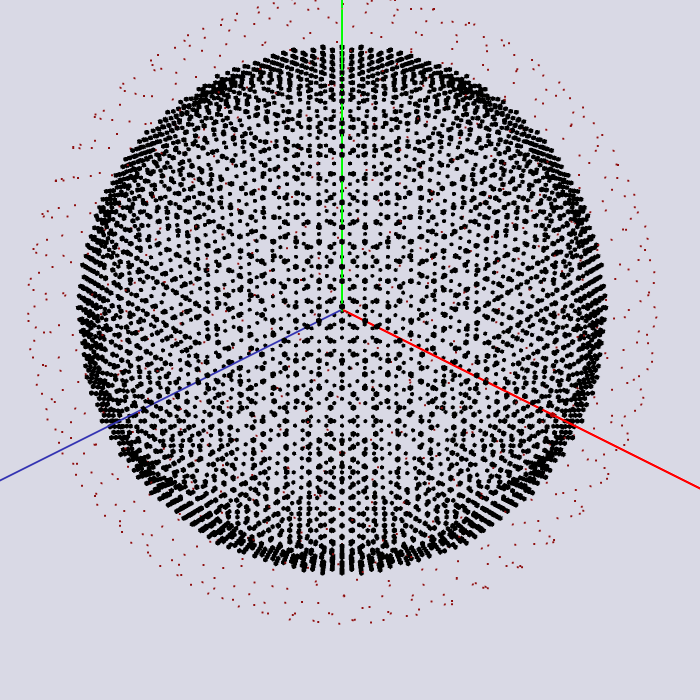
\includegraphics[width=0.7\linewidth]{fig_snapshot}
\end{center}
\caption{Emergent spherical wavefront. \label{fig:snapshot} Snapshot of the active shell (bright cells) propagating from a source centre; the front advances exactly one cell per tick, i.e. at the maximum information speed $v_{\max}$.  The red sphere of Fibonacci points delimits only the visual boundary of the spherical cavity (the radial dead zone at $r=\mathrm{RMAX}$ of Sect.~\ref{subsec:proof-of-concept}); it is not part of the simulation state.}
\end{figure}

\paragraph{Scattering.} A controlled head-on experiment (\texttt{scatter\_main.cpp} of Ref.~\cite{af_neto}) places two bubbles in layers $0$ and $1$ a distance $4$ apart with prescribed, opposite momenta $m=(+1,0,0)$ and $m=(-1,0,0)$ and complementary charge words ($0\text{x}00$ and $0\text{x}3F$, a Rule~1 pair), then runs $200$ light frames.  The two wavefronts overlap in $6{,}996$ cell-frame events, but the electroweak sieve gate $s2B$ admits only $18$ of them ($0.26\%$), and none of those triggers the pair-formation branch of the convolution; the bubbles keep their initial kinds and end at their starting positions (no deflection, total momentum conserved at zero).  This is a quantitative null result: at the amplitudes and clock scales of the small lattice, the probabilistic $s2B$ sieve essentially gates off the electroweak channel, which is the concrete mechanism behind the $\mathrm{form}=0$ of the charge census.  Scattering at observable rates would require larger amplitudes or a coarser $s2B$ threshold; with the current parameters the convolution channel is dormant.  Figure~\ref{fig:scatter} shows the two approaching wavefronts at contact.

\begin{figure}[ht]
\begin{center}
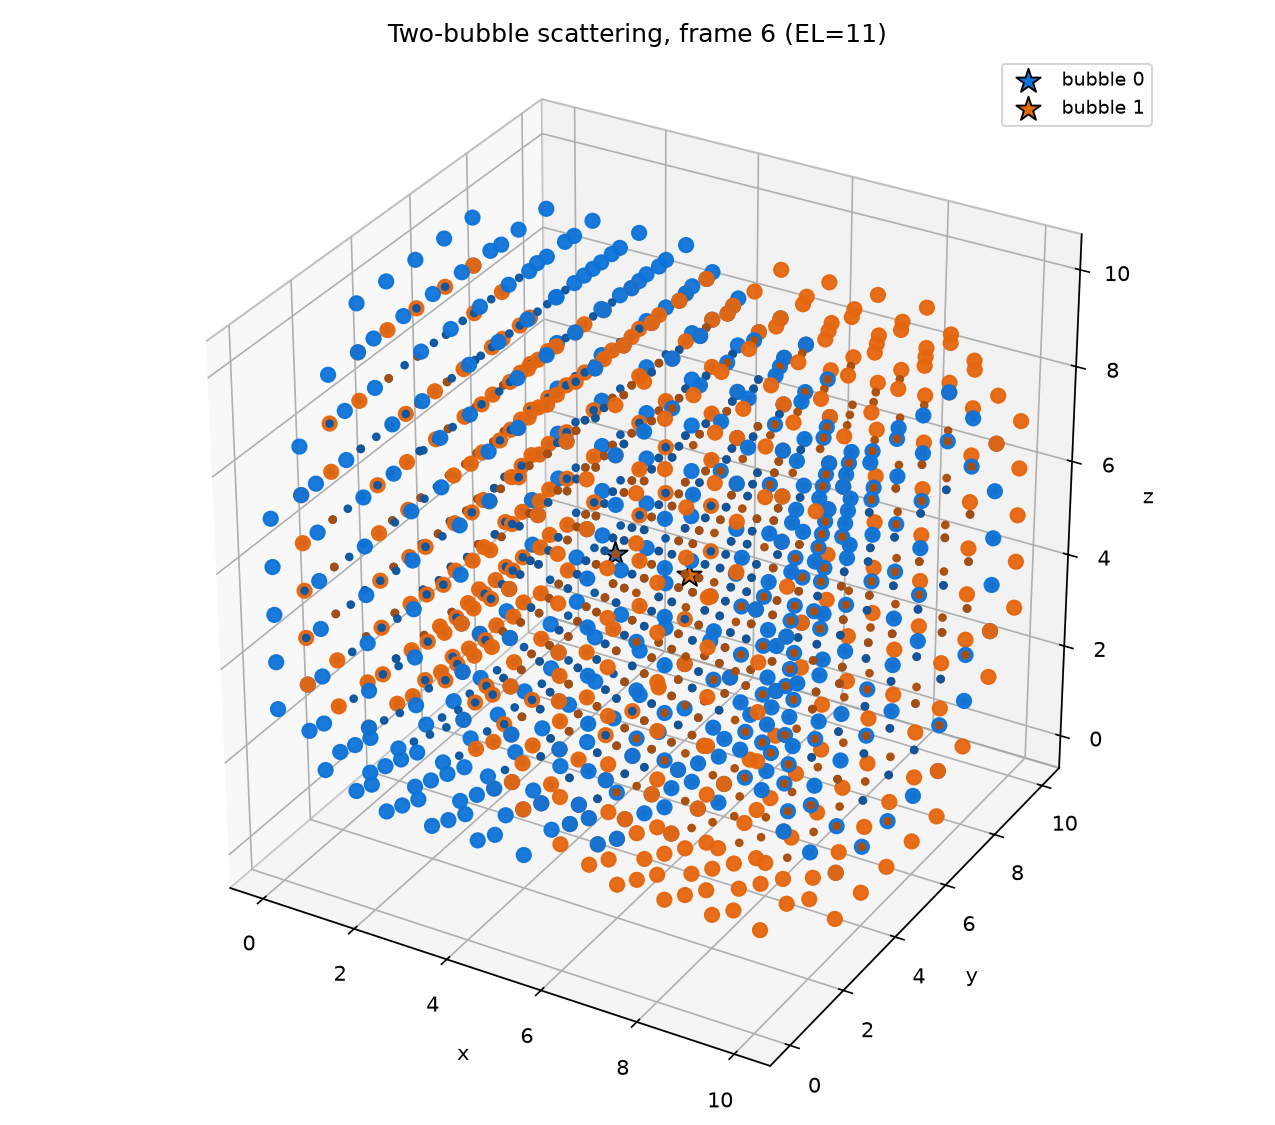
\includegraphics[width=0.7\linewidth]{fig_scatter}
\end{center}
\caption{Controlled head-on scattering. \label{fig:scatter} 3D voxel rendering of the two wavefronts (blue: bubble~0, orange: bubble~1) at the frame of closest approach; bright markers are the active shells.  The bubbles carry complementary charge words ($0\text{x}00$ and $0\text{x}3F$, a Rule~1 pair) and opposite momenta.  With the current amplitudes the $s2B$ sieve admits fewer than $1\%$ of overlaps and no pair branch fires (quantitative null result, see text).}
\end{figure}

\paragraph{What is not yet measured.}  Wavefront geometry and amplitude fidelity, charge conservation, bound-state stability and a controlled two-bubble scattering attempt are now reported above.  Still absent is a scattering event at an observable rate, which requires the $s2B$ gate to fire; claims in this manuscript that rely on frequent particle collisions should be read accordingly.

The next section discusses remaining challenges and limitations.

%%%%%%%% CELLULAR AUTOMATA AND QUANTUM FORMALISM %%%%%%%%%%

\section{Cellular automata and quantum formalism} \label{sec:bridge}

For local events, we follow 't Hooft's cellular-automaton world-model approach \cite{thooft}. Ontological CA states ($\mathcal{OS}$) do not superpose: each evolves into another ontological state. An orthonormal set of ontological states can nevertheless serve as a Hilbert-space basis.

The general operator-mechanics recipe is:

\begin{itemize}
    \item Find a permutation operator as a matrix containing a single 1 in any row or column.
    \item Diagonalize it, obtaining the eigenvalues and eigenvector matrices.
    \item Identify a Hamiltonian matrix as the exponent in $\hat{U}=e^{-i\hat{H}T}$.
    \item Use the eigenvalue matrix to bring this Hamiltonian back to the ontological basis.
    \item Form linear combinations of the ontological states $\ket{A}$.
\[
\ket{\psi} = \sum_A \lambda_A \ket{A}, \quad \sum_A |\lambda_A|^2 \equiv 1,
\]
where $\ket{\psi}$ is a quantum state or "template," and $\lambda_A$ is a complex coefficient.
\end{itemize}

With this operator machinery, the Schrödinger equation governs the deterministic evolution of the wave function:

\[
\frac{d}{dt}\ket{\psi} = -i\hat{H}\ket{\psi}.
\]

The Born rule follows once superposition states are accepted; it predicts the final eigenstate after measurement. This is a simplified picture; details are in \cite{thooft,Elze2019,rizzo2020perturbing}.

%%%%%%%% PROSPECTS AND CONJECTURES %%%%%%%%%%

\section{Conjectures and prospects\label{sec:Prospects-and-conjectures}}

The small-lattice implementation of Sect.~\ref{subsec:proof-of-concept} demonstrates only the mechanisms listed there: wavefront propagation, the integer-only polarization pair, W-island aggregation, and the charge census.  Everything discussed below is an \emph{interpretive conjecture} about how those mechanisms might behave at large $L$; none of it has been produced by, or tested against, the current implementation.  To keep the evidential status explicit, each topic is marked as either a \emph{structural analogy} (a mapping suggested by the six-bit charge algebra, with no dynamical output) or a \emph{speculative projection} (an extrapolation to a regime the implementation cannot reach).

\subsection{Discrete to continuous transition}

Localized particles are conjectured to be assemblies of many discrete fragments, so macroscopic properties such as total momentum and angular momentum might emerge from collective configurations rather than from individual bubbles. These global quantities would then be best described by real numbers, just as statistical mechanics bridges discrete atomic events to continuous thermodynamic variables.

A free electron's average motion, for example, may follow a direction vector that cannot be expressed with only discrete modulo-$L$ components; continuous descriptors are thus necessary idealizations at large scales. The same holds for isotropy: it looks uniform at macroscopic scales even though the lattice is fundamentally granular.

\subsection{Color quantization}
Color quantization is presented as an extension of the electromagnetic case. 
Hadrons would form by the simultaneous action of charge quantization and strong cohesion, producing color-neutral bound states of quark and gluon fragments. In the discrete color code (Sect.~\ref{subsec:specialized-pairs}), a strongly neutral combination would be either a pair of complementary color bits (meson-like), a pair of identical non-trivial colors (diquark-like), or a triplet of the three distinct colors (baryon-like, e.g.\ a proton $uud$ fragment). Free quarks would then be unobserved because only these color-neutral composites would be dynamically stable, any uncompensated color being rapidly balanced by quark-gluon exchange. This is a structural conjecture about the charge code; no hadron formation has been simulated.

\subsection{Special relativity}\label{subsec:special-relativity}
The measurement prescriptions for time intervals, spatial separations and clock synchronization \emph{follow those of} Einstein's special relativity \cite{Einstein1905} as a \emph{reading convention}: time is read by ideal clocks, distances by round-trip light-travel times, and coordinate time by a network of synchronized clocks. This convention describes how an external observer interprets the automaton output; it is not a symmetry of the transition rule, which evolves on a fixed lattice with a single global clock.

This is precisely the sense in which the speed of light is emergent in this model. The transition rule contains a single fundamental velocity, the maximum information speed $v_{\max}$ of Sect.~\ref{sec:Results} (one cell per tick), and knows nothing of light. An Observer (Sect.~\ref{subsec:observers}) that lays down synchronized clocks and measures distances by round-trip light signals \emph{reads} the photon of Sect.~\ref{subsec:pairs}---a pair of bubbles riding the wavefront---as moving at $v_{\max}$ and names the resulting constant $c$. A different observer structure would in principle read a different value; $c$ is therefore a property of the measuring structure, not of the rule.

As a purely formal, heuristic device for illustration---and only as such---the internal coordinate $W$ can be treated as a fourth spatial dimension, where the now 4D-bubbles form a thin shell, to avoid known 4D mutual passing issues (see Machotka \cite{Machotka2025}).  This construction plays no role in what follows: the time-dilation formula is derived kinematically from two ingredients of the automaton, both verified or constructed in the simulator:

\begin{enumerate}
  \item \textbf{Velocity independence and isotropy of the two-way speed.}  The active shell advances exactly one cell per tick at $v_{\max}$ from its source centre, independent of the source momentum and direction (Sect.~\ref{sec:Results}).  The round-trip Michelson--Morley probe (Sect.~\ref{subsec:lorentz-probes}) measures the front advance as $1.0000\pm0.0000$ cells/frame for source speeds $V=0$, $+1$ (axes $x$, $y$, $z$, and the diagonal $x{+}y$), $+2$, and $+3$, verifying the velocity-independence condition~1 of Mansouri and Sexl \cite{mansouri-sexl}.
  \item \textbf{Clock hypothesis.}  The bubble clock---the breathing phase $f=\mathrm{effective\_t}(t)$ of a source centre, a triangle wave of period $L$ frames---advances once per light frame for every cell, independent of its state of motion: the tick $t$ is the global frame counter, not a dynamical variable (Sect.~\ref{subsec:observers}).
\end{enumerate}

Consider a light clock: a free photon (Sect.~\ref{subsec:pairs}) bouncing between two mirrors (bubble boundaries) held at separation $D$, with the mirror axis perpendicular to the motion.  At rest, one tick is a round trip $2D$ at speed $v_{\max}$, so
\begin{equation}
\Delta\tau = \frac{2D}{v_{\max}} .
\label{eq:tick-rest}
\end{equation}

Moving at speed $v$ in the lattice frame, the clock translates by $v\,\Delta t$ during the tick $\Delta t$; the photon follows the diagonal path of total length $2\sqrt{D^{2}+(v\,\Delta t/2)^{2}}$, still at speed $v_{\max}$ (ingredient~1):
\begin{equation}
v_{\max}\,\Delta t \;=\; 2\sqrt{ D^{2} + \left(\frac{v\,\Delta t}{2}\right)^{2} } ,
\label{eq:lightclock}
\end{equation}
which gives, for the tick interval measured by the at-rest clock network,
\begin{equation}
\Delta t \;=\; \frac{\Delta\tau}{\sqrt{1-v^{2}/v_{\max}^{2}}} \;\equiv\; \gamma\,\Delta\tau , \qquad \gamma = \left(1-\frac{v^{2}}{v_{\max}^{2}}\right)^{-1/2}.
\label{eq:timedilation}
\end{equation}

The Observer reads the photon as moving at $c=v_{\max}$ (Sect.~\ref{subsec:observers}); with this identification Eq.~\eqref{eq:timedilation} is the time-dilation formula of special relativity,
\begin{equation}
\Delta\tau \;=\; \sqrt{1-\frac{v^{2}}{c^{2}}}\,\Delta t ,
\label{eq:timedilation-sr}
\end{equation}
derived from the two ingredients above instead of from the bookkeeping identification $\delta w=c\,\delta\tau$ used in earlier versions of this work.  By the clock hypothesis (ingredient~2) the same factor applies to any bubble clock, not only to light clocks: the intrinsic tick is motion-independent, and only its round-trip light measurement dilates.

The derivation uses only the round-trip convention: the light path is closed (out and back), so no one-way speed or simultaneity convention enters; the single measured input is the two-way speed, verified as $v_{\max}$ by the Michelson--Morley probe.  The dilation is therefore a \emph{reading} of the automaton output by the Observer's conventions, not a symmetry of the transition rule.

We emphasize that this is a kinematic derivation, not a Lorentz-invariance claim.  The lattice has no Lorentzian light cone---only the information cone at $v_{\max}$---and the transition rule is not invariant under Lorentz boosts.  Equation~\eqref{eq:timedilation} follows from the two ingredients alone, both verified in the simulator; it does not imply that the full particle dynamics are Lorentz invariant, which the present implementation does not test.  The field substrate does not enter the light clock: its plane-wave modes travel at $v_{\mathrm{wave}}=v_{\max}/2^{s/2}<v_{\max}$ (dispersion probe, Sect.~\ref{subsec:lorentz-probes}), strictly below the causal boundary, and cannot transmit a signal faster than $v_{\max}$.

\subsection{Lorentz probes in the simulator}\label{subsec:lorentz-probes}
Two numerical probes (test programs \texttt{lorentz\_mm.cpp} and \texttt{dispersion.cpp}, this work) quantify how the lattice dynamics approach Lorentz symmetry at low energies.

\paragraph{Michelson--Morley (two-way isotropy).}  The probe seeds a source centre and measures the advance of the active-shell front per light frame, exactly as the wavefront instrumentation of Sect.~\ref{sec:Results}.  For a source at rest ($V=0$), a source given constant momentum $V=+1$ along $x$, $y$, $z$ and the diagonal $x{+}y$, and sources with $V=+2$ and $+3$, the measured advance is
\begin{equation}
\frac{\Delta r_{\mathrm{front}}}{\Delta t} \;=\; 1.0000 \pm 0.0000 \ \mathrm{cells/frame},
\label{eq:mm-front}
\end{equation}
i.e., the two-way round-trip time of the shell is isotropic and source-independent at the resolution of the probe.  This verifies the velocity-independence condition~1 of Mansouri--Sexl \cite{mansouri-sexl} and is the empirical anchor of ingredient~1 of the time-dilation derivation (Sect.~\ref{subsec:special-relativity}).

\paragraph{Dispersion (linear low-energy regime).}  The probe seeds a standing plane wave $u=A\cos(kx)$ on the substrate field and counts zero crossings at the origin to measure $\omega(k)$ (integer arithmetic, $A=2^{20}$; negligible damping).  The measured relation matches the analytic dispersion of the discrete wave equation,
\begin{equation}
\omega(k) = \arccos\!\left(1-\frac{\lambda}{2^{s+1}}\right), \qquad \lambda = 4\sum_{i}\sin^{2}\!\frac{k_{i}}{2},
\label{eq:dispersion}
\end{equation}
to four to five decimal places across the Brillouin zone.  At small $k$ the dispersion is linear,
\begin{equation}
\omega \;\approx\; v_{\mathrm{wave}}\,k , \qquad v_{\mathrm{wave}} = \frac{1}{2^{s/2}} ,
\label{eq:wave-speed}
\end{equation}
with measured slopes $0.248$, $0.175$ and $0.125$ for integer shifts $s=4,5,6$, against the analytic $0.2500$, $0.1768$ and $0.1250$.  The lattice corrections bend the dispersion near the Brillouin boundary ($\omega/k$ falls by $\approx35\%$ at $k=\pi$ for $s=5$); the leading deviation from linearity is quadratic in $k$,
\begin{equation}
\frac{\Delta\omega}{\omega} \;\approx\; -\frac{k^{2}}{24},
\label{eq:dispersion-correction}
\end{equation}
the generic suppression of Lorentz symmetry by the square of the lattice (Planck) scale.  The substrate wave speed $v_{\mathrm{wave}}$ is strictly subluminal with respect to $v_{\max}$: the field cannot be used to exceed the causal boundary.  In the model the integer shift varies radially ($s=\mathrm{DIFF\_SHIFT}+1-(r\gg\mathrm{diffDivShift})$, clamped), so $v_{\mathrm{wave}}$ acquires a radial profile; the probe uses a constant shift $s$ to isolate the intrinsic dispersion of a homogeneous substrate.

\subsection{Emergence of gravity}\label{subsec:emergence-of-gravity}

General-relativistic spacetime is here conjectured to be an effective, coarse-grained approximation of the discrete lattice (a speculative projection). Gravity is proposed to arise as a residual effect of electromagnetic interactions, mediated by the gravitons of Sect.~\ref{subsec:specialized-pairs}---pairs with fully complementary charge words---which couple to both \emph{Orbis} and \emph{Umbra}. Ordinary photons are sector-specific, but gravitons provide cross-sector connectivity; being charge-neutral by construction, a graviton's electric and weak contributions cancel at leading order, leaving a residual geometry-driven attraction. Under this conjecture, free objects would follow emergent timelike geodesics under the Observer's round-trip reading convention (Sect.~\ref{subsec:observers}), and graviton redistribution of energy and charge might mimic dark-matter effects such as flat rotation curves. None of these behaviours has been observed in the implementation.

In the same coarse-grained picture, photons may also lose energy through minor, non-collapsing interactions with singletons and electrons as they propagate---an intrinsic \textit{aging} that would parallel cosmic redshift. In the model a photon's frequency is an integer pair population (Sect.~\ref{bosons}), so each interaction that removes one pair lowers the emergent frequency read by an Observer by one quantized even step. Zwicky already proposed a redshift mechanism independent of expansion \cite{zwicky1929redshift}; in principle the model could realize it without the image-blurring problem he raised, offering a redshift explanation that does not require dark energy. The propeller mechanism of Sect.~\ref{subsubsec:propeller} might likewise make acceleration equivalent across frames, in line with the equivalence principle. These are suggestions, not measured effects.

\subsection{Weak quantization}
Because weak interactions are rare, weak quantization may appear at cosmological scales, for instance in a constant ratio between the average galaxy separation and galactic bulge size. This large-scale granularity could be reinterpreted as gravitational quantization and may eventually yield an effective cosmological constant $\Lambda$ and metric tensor $g_{\mu\nu}$.

\subsection{Stochastic behavior and the uncertainty principle}

The initial chaos created by the deterministic collision of many regular patterns, together with the large number of bubbles per particle, may make individual outcomes effectively unpredictable. Each measurement would then sample one instance from this fine-grained distribution, so measured values could carry irreducible uncertainty, analogous to the Heisenberg principle \cite{Heisenberg1927}:

\[
\sigma_x \sigma_p \leq \frac{\hbar}{2}.
\]

\subsection{Black holes}
The quintessential idea of a black hole in this model can be illustrated by two electrons, each with radius $R$, so close to each other $d<2R$ that the quantization is broken and they simply fuse, forming a particle with radius $R'=2^{1/3}R$ with a dominant affinity value. 
\[
a_1 = a_2 = \min(A_1,A_2).
\]

The toy picture above contains no mechanism that would obviously discard information; this is, however, not a resolution of the black hole information paradox \cite{hawking1976breakdown,harlow2016jerusalem}, and no black-hole dynamics has been simulated in this framework.

\subsection{What is spin in this model?}
In this model, spin is conjecturally identified with the coherent radial alignment of the pBit $pB$ (local in-phase sign) and the transverse polarization pair $(\mathrm{pol}_u,\mathrm{pol}_v)$. The positive in-phase half-cycle marked by $pB$ alternates outward and inward as the wave oscillates, while the phase of $(\mathrm{pol}_u,\mathrm{pol}_v)$ winds once around the wavefront. This radial helix would define the two spin states, aligned consistently across the particle's constituent bubbles. This identification is a structural conjecture; the model's spin has not been measured against Stern–Gerlach-type experiments.

\subsection{The Hofer effect}\label{subsec:hofer}

A key test would be the \emph{Hofer effect}: the predicted tendency of all individual spins of a localized particle to align radially inward or outward (spin down/up). Hofer \cite{hofer} argues that magnetic effects arise from breaking the spherical symmetry of this pattern, offering an interpretation of the Stern–Gerlach experiment. Whether the model reproduces this effect is not yet demonstrated.

\subsection{Particle zoo panorama}
As a heuristic exercise, this model offers a framework to speculate on the composition of known particles; the identifications below are structural analogies based on the six-bit charge code, none produced by the small-lattice implementation. 
In the discussion that follows, the fragments will be characterized by their charge content: \(q, w1, w0, c2, c1, c0\). 
For example, we designate the fragment \(100000\) as \(-L\) and \(001111\) as \(-\bar{L}\), and so forth. 
Whether these compositions actually occur under the evolution rules is not demonstrated by the current implementation; it remains to be established by future simulations.

\subsubsection{The electron neutrino}
The electron neutrino $\nu_e$ is conjectured to be formed by a single [$+L:-L$] pair and additional propellers. 
Yet the anti-electron neutrino $\bar{\nu}$ would use the pair [$+\bar{L}:-\bar{L}$].

\subsubsection{The electron}
The electron $e^-$ is conjectured to be formed by a quantized number of $-L$ fragments, a great number of electron neutrinos $\nu_e$, and a variable number of propellers (see Figure \ref{fig:electron}). The positron, or anti-electron, would use $+\bar{L}$ fragments instead. These are for Orbis, in the case of Umbra, all bits are inverted.

\begin{figure}
\begin{center}
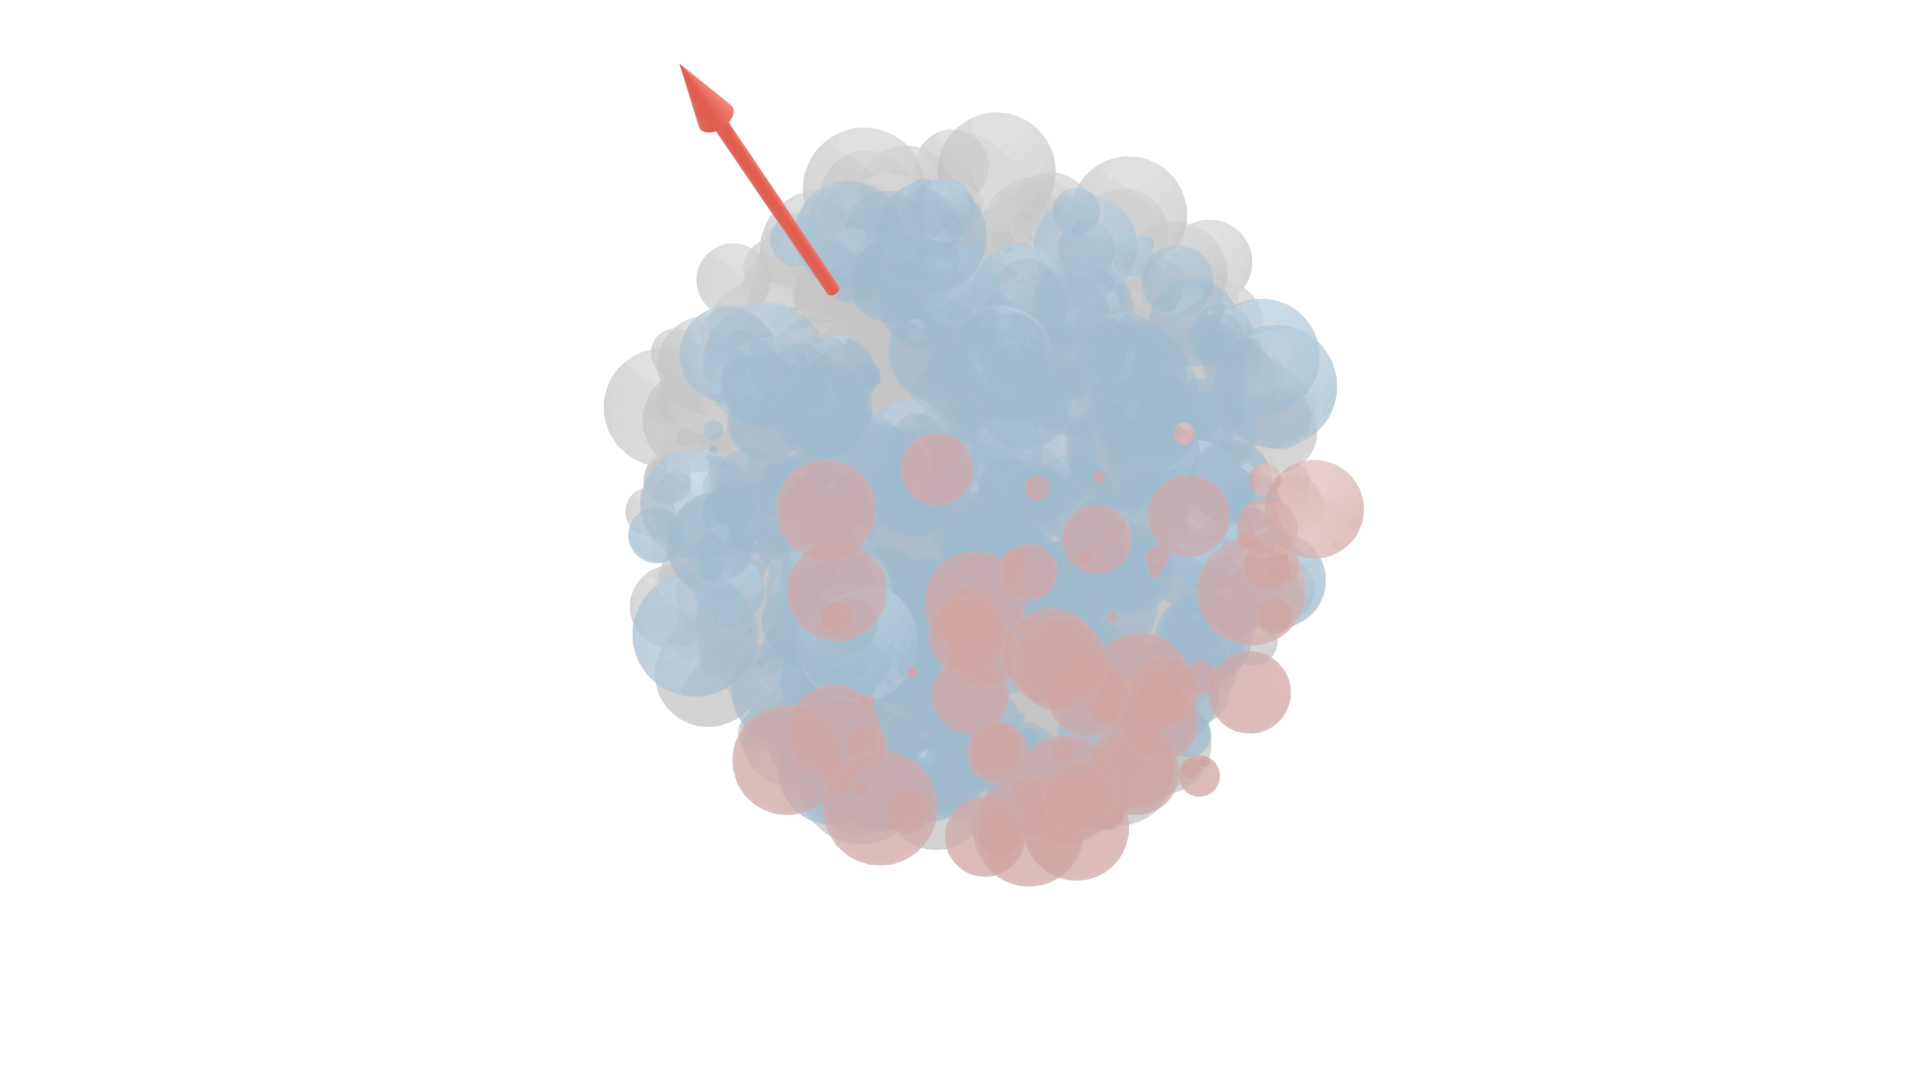
\includegraphics[width=\linewidth]{fig3}
\end{center}
\caption{The free electron.}
\footnotesize{Artistic impression of a free electron. The red bubbles are propellers with a resultant in the direction of the arrow. The blue bubbles are negative charge singletons, while the gray bubbles are electron-neutrino pairs.}
\label{fig:electron}
\end{figure}

\subsubsection{The muon neutrino}
The muon neutrino $\nu_{\mu}$ is conjectured to be formed as $\nu_{\mu}=2\nu_e+\bar{\nu}_e$ plus additional propellers. 
It would be like an electron neutrino, but with a compensated antimatter part.

\subsubsection{The muon}  
The muon $\mu^-$ is conjectured to consist of a quantized number of $-L$ fragments, a large number of muon neutrinos $\nu_{\mu}$, and a variable number of propellers. 
The classical study conducted by Itô in \cite{ito} suggests that this configuration stabilizes at the second harmonic of the electron's radial vibrational state.

\subsubsection{The tau neutrino}
The tau neutrino $\nu_{\tau}$ is conjectured to be formed as $\nu_{\tau}=3\nu_e+2\bar{\nu}_e$ plus additional propellers. 
It would also be like an electron neutrino, but with a compensated antimatter-enriched part.

\subsubsection{The tau}
The tau $\tau^-$ is conjectured to be formed by a quantized number of $-L$ fragments, a great number of tau neutrinos $\nu_{\mu}$, and a variable number of propellers.

\subsubsection{Gauge bosons}
These bosons were described in Sect. \ref{bosons}.

\subsection{Leptons decay}
In the Standard Model (SM), the decay products typically include one neutrino or antineutrino.
In our model, one might conjecture that the large number of neutrinos in a particle is entangled by a common affinity, so that when one neutrino interacts via the weak force, all other entangled neutrinos collapse to the same point.
Under that conjecture, the observable outcome would be indistinguishable from a single, energetic neutrino, in agreement with the SM prediction.
If the neutrino belongs to the other sector (Orbis/Umbra), spontaneous decay might follow.  None of this behaviour has been observed in the implementation.

\subsection{Electronic decay}
After the absorption of (part of) a photon, the electron would, under the model, enter an excited state, dynamically stabilizing in a suitable spherical harmonic configuration. 
When the common components of the photon and electron are reissued, the odds of a configuration corresponding to the original photon are less than one. 
As time passes, after many cohesion interactions, the proper configuration of charges and pBits may occur, forming a single photonic blob and allowing the emitted photon to escape the frequent reissue mechanism, fleeing away from the electron cloud, which eventually settles into its ground state.

\subsection{Compound particles half-lives}
Protons, electrons, and electron neutrinos are, under the model, composed exclusively of bubbles, without their corresponding anti-bubbles. 
This unique composition is offered as a key factor in their exceptionally long half-lives, potentially making them stable. 
In contrast, particles containing both bubbles and anti-bubbles are conjectured to be significantly less stable. 
Their shorter half-lives would result from the likelihood of annihilation events between bubbles and anti-bubbles within their structure, leading to their transient nature.

The neutron would, under the model, embed lots of electron antineutrinos, which bind the negative charge to its inner proton. 
This is offered as a possible explanation of the free neutron decay.
\[
n^0\rightarrow\,p^{+}+e^{-}+\nu_e
\]

\subsection{Nuclear decay}

In this model, nuclear decay processes emerge from the internal structure and composition of compound particles representing atomic nuclei. 
These instabilities trigger reorganizations via the electroweak collapse mechanism, where the sieve test result ($s2B$) determines the feasibility of transformations. 
The decay process is similar to the free neutron decay seen above. 
The perturbing particles are typically neutrinos and Z bosons that permeate the vacuum. Once again, if these perturbing particles belong to the other sector (Orbis/Umbra), then we have spontaneous decay.

This internal annihilation mechanism is offered as a possible account of decay processes; whether it reproduces the empirical tables of nuclides is not established, since no nuclear-scale configuration has been simulated.

\subsection{Heavier quarks}
The framework speculatively suggests that the other quarks could follow the composition of leptons, with additional neutrinos and antineutrinos, besides a variable number of propellers.

\subsection{Atoms}
Bound states of protons, neutrons, and electrons might naturally be expected in this scenario; their formation is not demonstrated by the current implementation.

\subsection{The abundance of neutrinos}

Despite the relatively small number of neutrinos observed in Table \ref{tab:color-combination}, their large cosmic abundance reflects their low mass, approximately five million times smaller than the mass of an electron. 
This characteristic allows neutrinos to exist in enormous quantities across the universe, even if their presence appears limited.

\subsection{Partons}
The inertia mechanism adopted here implies that the collective action of a large number of identical propellers produces a high‑energy configuration. This stretches the propelled mass along the direction of motion, thereby forming a \textit{parton} structure.

\subsection{Quest for qubits} \label{subsection:qubits}

An electron may be conceived as a vast ensemble of dynamic \textit{nanostates}, collectively manifesting as a single particle through their shared affinity. 
When two electrons share the same affinity (totally or partially), they become distinguishable only through the constraints imposed by quantization dynamics. 
However, if one momentarily relaxes these constraints, such a pair could in principle be interpreted as a system of qubits; this is a speculative reading, not a demonstrated computational capability.

What, then, supports this emerging computation? 
Spatial interaction is facilitated by the convolution step, while the self-interference mechanism (see Sect.~\ref{subsec:Interference}) introduces a form of temporal smearing that allows information to persist and influence future states.

Moreover, the atoms that host these electron structures local space via the SU(3) symmetry induced by the strong charge, further enriching the landscape of possible interactions.

This broader perspective suggests a behavior akin to an intricate network of Turing machines, each representing a potential computational pathway. 
The computation results are being revealed by interpreting correlations. 
Such an interpretation might offer insight into quantum computing, but no computation has been performed in this framework.

\subsection{Observers and spacetime}\label{subsec:observers}  

This framework extends Wheeler's "it from bit" concept by providing a mechanism through which information constitutes physical entities, albeit from an omniscient perspective. 
To address the internal viewpoint, we now define inner observers or simply \textit{observers}. 

\subsubsection{Minimal observer definition}

Here, we formalize the concept of a \emph{minimal observer}, following the framework introduced in Hatem Elshatlawy et al. \cite{elshatlawy2025towards}. 
A minimal observer is defined as the simplest system capable of performing observation in a functional sense, embodying core components of sensing, internal processing, and acting upon an environment within a closed feedback loop.

\begin{definition}[Minimal Observer]
Let $O$ be a system described by the tuple
\[
O = (X, Y, Z, f, g, B),
\]
where:
\begin{itemize}
    \item $X$: Internal state space (e.g., memory or configuration states),
    \item $Y$: Input (sensor) space,
    \item $Z$: Output (action) space,
    \item $f: X \times Y \rightarrow X$: State transition function (state update rule),
    \item $g: X \rightarrow Z$: Output function (generates actions based on internal state),
    \item $B$: Boundary condition demarcating the internal observer from its external environment.
\end{itemize}

The system $O$ qualifies as a \emph{minimal observer} if it satisfies:
\begin{itemize}
    \item $|Y| \geq 1$: Non-trivial sensing,
    \item $|Z| \geq 1$: Non-trivial actuation,
    \item $|X| > 1$: Non-trivial internal dynamics,
    \item \textbf{Feedback closure:} The output $g(x)$ must influence the environment in such a way that it alters future inputs $y \in Y$.
\end{itemize}
\end{definition}

This definition ensures that the observer possesses the minimal necessary structure to distinguish itself from its environment and engage in interaction through perception and response. 
Importantly, this framework abstracts away from higher-order capabilities such as memory, learning, or consciousness, focusing instead on the foundational structure that enables observation.

\subsubsection{Spacetime}
As established, the spacetime of this model is inherently flat and regular. 
One may conjecture that the spacetime perceived by observers and laboratory instruments would nevertheless appear curved, in analogy with General Relativity. 
How can this apparent discrepancy be reconciled?  

A proposed resolution lies in the role of propellers, which contribute both to motion and to mass-energy content. 
Their interactions create a framework in which observers, laboratory instruments, and the environment mutually influence one another. 
If their interactions generated effective potentials, clocks would tick slower near concentrations of mass. 
Whether this actually reproduces the \textit{timescape} scenario \cite{duley2013timescape}—curved spacetime emerging from relational dynamics in a flat background—is an open conjecture that the current implementation cannot test.


Within this framework the speed of light acquires a precise ontological status. The fabric possesses exactly one fundamental velocity, the maximum information speed $v_{\max}$ of Sect.~\ref{sec:Results} (one cell per tick). When a minimal observer measures intervals by the round-trip convention of Sect.~\ref{subsec:special-relativity}, the emergent photon is found to travel at this speed, and the observer names the ratio $c$; nothing in the transition rule refers to $c$. The essentially superluminal processes of the automaton---convolution and the other globally coordinated sweeps---are invisible to this measurement: they transfer no information, cannot be used to send messages, and cannot be manipulated by any observer. Causality is thereby protected: every influence an observer can emit or detect propagates at or below $v_{\max}$, so no signal ever arrives before it is sent.

Given the mutual dependence of all system components and the absence of free external variables, one might speculate that the model, if interpreted as a complete physical theory, would align with superdeterministic readings of reality as discussed by Hossenfelder and Palmer \cite{hossenfelder2020rethinking}.

%%%%%%%% CONCLUSION %%%%%%%%%%

\section{Conclusion\label{sec:Discussion}}

\subsection{Undecidability and long-term dynamics}\label{sec-undecidability}

Long-term dynamics involve Poincaré cycles. Because the CA can be Turing-equivalent, questions about recurrence versus chaos are undecidable in general \cite{wolfram1983,gacs1979}. The finite state space guarantees eventual recurrence (Pigeonhole principle), but the configuration space grows exponentially with $L$, making detection infeasible \cite{bernstein2007,toffoli1980}. Affinity further stretches the probable recurrence time: by binding bubbles into persistent particles and aligning them into long-lived 3D islands, it reduces the effective number of independently evolving configurations and channels the dynamics through organized attractors rather than allowing rapid, unstructured mixing. Black-hole fusion may then absorb exceptional configurations (`Gardens of Eden') and drive the system toward a Poincaré cycle. Undecidability limits algorithmic predictability, so analytical tools are needed for general insights.

\subsection{Falsifiability of the physical model}

A direct observation that an electron physically traverses both paths in a double-slit experiment would contradict the model. Self-interference here arises from recorded lattice traces, not from simultaneous path occupation. 

\subsection{Novelty of the work}

Compared with prior work surveyed in Sect.~\ref{sec:related-work}, this model introduces four main novelties:
\begin{enumerate}
  \item A non-spatial dimension $W$ that acts as a dynamic computational layer, enabling cross-layer convolution---a superluminal but strictly non-signaling and non-manipulable update mechanism that protects causality---and richer interactions than Zuse's purely spatial ``digital particles.''
  \item Six charge bits per cell, giving Lie-group-like symmetries and Noether-like conservation at a programmable level.
  \item Affinity, which groups bubbles into particles and encodes self-interference histories.
  \item Ontological collapse events that break strict reversibility within a Poincar\'{e} cycle, matching the effective irreversibility of quantum measurement.
\end{enumerate}
The model retains a discrete lattice while capturing quantum and relativistic features; it remains exploratory and must still be validated against empirical data.

\subsection{Limitations and open problems}

For clarity, we collect here what the current implementation cannot yet do.  These are structural limitations of the code as it stands (small lattice, dormant electroweak gate), not of the model idea; each is stated with the corresponding evidence from Sect.~\ref{sec:Results}.

\begin{itemize}
  \item \textbf{No true multi-particle bound states yet.}  The in-simulation census registers no pair formation at all ($\mathrm{pairM}=\mathrm{pairA}=0$, $\mathrm{form}=0$, $\mathrm{blob}=0$; Sect.~\ref{subsec:proof-of-concept}), and the controlled two-bubble experiment yields a quantitative null result: of $6{,}996$ overlapping cell-frame events only $18$ ($0.26\%$) pass the $s2B$ sieve and none triggers the pair branch.  Bound states such as hadrons and atoms therefore remain conjectural; the aggregates that do persist (the $1K+nD$ islands of Sect.~\ref{sec:dynamic-charge-quantization}) are affinity-driven populations, not charge-bound composite particles.
  \item \textbf{Continuum limit absent.}  The model is defined on a finite $3$-torus of side $L\le31$ with a single cell as the unit of length.  There is no procedure for taking $L\to\infty$ (or the cell size to zero), no coarse-graining scheme, and no derivation of a partial-differential or field-theory limit.  The $r\cdot\sin(r)$ wave cloud (Sect.~\ref{subsec:Sine}) is an emergent lattice pattern, not a solution of a continuum equation.
  \item \textbf{No quantitative comparison with measured cross-sections.}  No scattering amplitude, cross-section, or decay rate has been computed from the automaton; the single dimensionless number available ($m_{p}/m_{e}\approx1187$ vs.~the empirical $\approx1836$) is a kinematic census ratio, not a prediction derived from the interaction rules.  Units are defined only up to the lattice scale $X$ (Appendix~\ref{sec:Calculation-of-X}); there is no mapping from cells-per-tick to physical velocities or energies.
  \item \textbf{Small-lattice and boundary effects.}  The reported runs use $L=7$ (Sect.~\ref{subsec:proof-of-concept}); the spherical cavity and the radial dead-zone at $r=\mathrm{RMAX}$ suppress corner artifacts by construction, but also truncate long-range phenomena.  The layer-symmetric seed makes all $75$ islands statistically identical, a configuration choice rather than a property of the dynamics.
  \item \textbf{Electroweak channel effectively dormant.}  The $s2B$ sieve admits fewer than $1\%$ of overlaps at the current amplitudes (Sect.~\ref{subsec:proof-of-concept}), so weak phenomena---neutrino interactions, $W/Z$ fragments, decay chains, and the inter-sector rules of Sect.~\ref{subsec:distinct}---are described by the algorithms of Sect.~\ref{subsec:algorithm} but have not been observed to fire in the automaton itself.
  \item \textbf{Open problems.}  (i)~Find parameter regimes in which the $s2B$ gate fires and pair formation is observed, and study the resulting bound states; (ii)~define a continuum limit and derive effective equations; (iii)~turn the charge-combination census into genuine cross-section predictions with a unit mapping; (iv)~scale the lattice to test multi-particle dynamics beyond two bubbles; (v)~derive the model constants ($U_{0}$, sieve thresholds, $\mathrm{phase\_full}$) rather than setting them by hand.
\end{itemize}

These limitations delimit the scope of the present work: the manuscript reports mechanisms and exploratory observations, not a predictive physical theory.  The conjectures of Sect.~\ref{sec:Prospects-and-conjectures} and the falsifiability discussion above should be read in this light.

\subsection{Future inclusions}

Ongoing work simulates the geometric structures that emerge from these local, multi-layered updates. Preliminary tests already show that the collective dynamics of fragments produce a continuous $r \cdot \sin(r)$ density cloud, localized wave-packets, stable spiral patterns and macroscopic rotations directly from discrete bit distributions. These observations support the conjecture that the universal fabric can bridge discrete local rules and the smooth symmetries of physical spacetime.

\subsection{Final thoughts}

The model is an economical ontological framework\footnote{Especially when contrasted with the Many-Worlds Interpretation of quantum theory \cite{everett1957}.} operating at a deep subatomic scale. Observable reality is approximate and emergent, with continuous spacetime symmetries (Lie, Lorentz, diffeomorphism, CPT, etc.) arising from the dynamics. Each particle is composed of an enormous number of bubbles—each a miniature universe—so intrinsic non-locality provides a natural substrate for superposition-like behavior and qubit analogs. The theory remains to be refined computationally and tested against experiment; whether it can become a predictive, falsifiable, \emph{bona fide} physical theory is an open question.

%%%%%%%% FUNDING %%%%%%%%%%

\section*{Funding and competing interests}
\begin{verbatim}
The author declares that no funds, grants, or other support were received 
during the preparation of this manuscript.

The author has no relevant financial or non-financial interests to disclose.
\end{verbatim}

\section*{Author contributions and AI disclosure}
\begin{verbatim}
During the preparation of this work, the authors used generative AI tools to
improve the readability and language, as well as to assist in debugging and
optimizing numerical algorithms. After using these tools, the authors reviewed
and edited the content as needed and take full responsibility for the content
of the publication.
\end{verbatim}

\printbibliography

\newpage{}

%%%%%%%% APPENDIX %%%%%%%%%%

\appendix
\begin{center}
{\LARGE{}Appendix}{\LARGE\par}
\par\end{center}

\section{Calculation of X and L\label{sec:Calculation-of-X}}

Estimates for the value of \emph{X} and the distance between the cells
and \emph{L} (see Sect. \ref{sec:space-and-time}), the granularity
of the grid, will be developed in this appendix.

Note that the calculations below are derivation-only: per the purity constraints (Sect.~\ref{subsec:purity}), real numbers serve solely as intermediaries to compute integer parameters and are never invoked inside the runtime transition rule.  The values of $X$ and $L$ obtained here are rounded to integers and used once at initialization as fixed topological data.

The empirical inputs used below---in particular the measured speed of light $c$ and the observed diameter of Eq.~\eqref{eq:obs}---are observer-measured quantities in the sense of Sect.~\ref{subsec:observers}: $c$ is the emergent speed read from the fabric's fundamental constant $v_{\max}=X/\mathcal{L}$ (Sect.~\ref{sec:Results}). The appendix therefore calibrates the cell scale $X$ and the lattice side $L$ against observed data without altering the transition rule.

The diameter of the observable universe \cite{halpbern} is compared
to the diagonal of the lattice.

\begin{equation}
O=8.8\times10^{26}m=\sqrt{3}\,L\cdot X.\label{eq:obs}
\end{equation}
The average photon frequency of CMB \cite{archeops} is

\[
[f]=160\,GHz=160\times10^{6}\,Hz,
\]
which, converted to energy, gives

\[
E=1.060171224\times10^{-25}J.
\]
The proton mass in Joules is

\[
m_{p}=1.503277592969\times10^{17}J,
\]
so, the number of average photons in a proton is

\[
n_{p}=1.4179573\times10^{42}.
\]
The Eddington number gives the number of protons in the universe.

\[
Ed=10^{80}.
\]
Let us calculate the total contribution due to protons in terms of
average photon

\[
n_{pT}=4\,Ed\,n_{p}
\]
or

\[
n_{pT}=5.67183\times10^{122}.
\]
On the other hand, the number of photons in the universe is

\[
n_{\gamma}=4\times10^{84},
\]
which adds almost nothing to the total number due to protons

\[
n_{\gamma T}=n_{\gamma}+n_{pT}=5.67183\times10^{122}.
\]
The wavelength of a single bubble in meters is

\[
\lambda_{0}=L\cdot X
\]
and the frequency of one bubble, in Herz reads

\[
f_{0}=\frac{c}{L\cdot X},
\]
helping to find the number of bubbles in the average photon

\[
n_{b}=\frac{[f]}{f_{0}}=\frac{160\times10^{6}\,L\cdot X}{c}.
\]
So, the amount of bubbles due to all photons is

\[
n_{bT}=n_{b}\,n_{\gamma T}=2\frac{5.67183\times10^{122}\times160\times10^{6}\,L\cdot X}{c}
\]
and

\[
n_{bT}=L^{3}.
\]
We then have

\begin{equation}
\frac{1814.9856\times10^{128}\,X}{c}=L^{2}.\label{eq:number}
\end{equation}
Using Eqn. (\ref{eq:obs}) and Eqn. (\ref{eq:number}), we obtain 

\[
X\approx7.52831\times10^{-24}m
\]
and

\[
L\approx6.74877\times10^{49}.
\]

Assuming that the Planck length is a valid length scale, let us recalculate
$Ed$ for $X=l_{p}$.

\[
Ed=\frac{\sqrt{3}\,c\,O^{2}}{1920\,n_{p}\,l_{p}^{3}}=2.18816\times10^{113}.
\]
Then we finally obtain

\[
X\approx1.616199\times10^{-35}m=l_{p}
\]
and

\[
L\approx6.95410\times10^{60}.
\]

%%%%%%%%%%%%%%%%%%%%%%%%%%%%%%%%%%%%%%%%%%%%%

\end{document}